\documentclass[lineno]{biometrika}
\usepackage{amsmath}
\usepackage{graphics}
\usepackage[colorlinks,citecolor=blue,urlcolor=blue]{hyperref}
\usepackage{color}
%% Please use the following statements for
%% managing the text and math fonts for your papers:
% \usepackage{times}
% \usepackage[cmbold]{mathtime}
\usepackage{bm}
\usepackage{bbm}
\usepackage{subcaption}
\usepackage{newtxtext}
\usepackage[subscriptcorrection]{newtxmath}
%\usepackage{natbib}

\graphicspath{{./figures/}}

\usepackage[plain,noend]{algorithm2e}

\makeatletter
\renewcommand{\algocf@captiontext}[2]{#1\algocf@typo. \AlCapFnt{}#2} % text of caption
\renewcommand{\AlTitleFnt}[1]{#1\unskip}% default definition
\def\@algocf@capt@plain{top}
\renewcommand{\algocf@makecaption}[2]{%
  \addtolength{\hsize}{\algomargin}%
  \sbox\@tempboxa{\algocf@captiontext{#1}{#2}}%
  \ifdim\wd\@tempboxa >\hsize%     % if caption is longer than a line
    \hskip .5\algomargin%
    \parbox[t]{\hsize}{\algocf@captiontext{#1}{#2}}% then caption is not centered
  \else%
    \global\@minipagefalse%
    \hbox to\hsize{\box\@tempboxa}% else caption is centered
  \fi%
  \addtolength{\hsize}{-\algomargin}%
}
\makeatother

%%% User-defined macros should be placed here, but keep them to a minimum.
\def\Bka{{\it Biometrika}}
\def\AIC{\textsc{aic}}
\def\T{{ \mathrm{\scriptscriptstyle T} }}
\def\v{{\varepsilon}}
% LaTeX macros

% Last modified: 24/2/2008


%----------------------------------------------
%  A. C. Davison, Institute of Mathematics,
%  EPFL, 1015 Lausanne, Switzerland
%  00 41 21 693 5502
%----------------------------------------------

% mathematical symbols, etc.

\def\half{{\textstyle{1\over 2}}}
\def\third{{\textstyle{1\over 3}}}
\def\quarter{{\textstyle{1\over 4}}}
\def\sixth{{\textstyle{1\over 6}}}
\def\frac#1#2{{\textstyle{#1\over#2}}}
\def\Beta{{\rm B}}

\def\argmin{{\rm argmin}}  
\def\diag{{\rm diag}}  
\def\mod{{\rm mod}}  
\def\tr{{\rm tr}}
\def\sign{{\rm sign}}
\def\ow{{\rm otherwise}}  
\def\obs{{\rm obs}}  
\def\endex{{\hfill{\color{red}$\bullet$}\medskip}}
\def\Endex{{\hfill{$\bullet$}\medskip}}
\def\redbf#1{{\color{red}\bf #1}}%
\def\red#1{{\color{red} #1}}%
\def\white#1{{\color{black} #1}}%

\DeclareSymbolFont{AMSb}{U}{msb}{m}{n}
\DeclareMathSymbol{\Natural}{\mathbin}{AMSb}{"4E}
\DeclareMathSymbol{\Integer}{\mathbin}{AMSb}{"5A}
\DeclareMathSymbol{\Real}{\mathbin}{AMSb}{"52}
\DeclareMathSymbol{\Rational}{\mathbin}{AMSb}{"51}
\DeclareMathSymbol{\Imaginary}{\mathbin}{AMSb}{"49}
\DeclareMathSymbol{\Complex}{\mathbin}{AMSb}{"43} 
\DeclareMathSymbol{\Disk}{\mathbin}{AMSb}{"44} 
\def\bi{\begin{itemize}}
\def\ei{\end{itemize}}
\def\bd{\begin{description}}
\def\ed{\end{description}}
\def\ben{\begin{enumerate}}
\def\een{\end{enumerate}}
\def\bv{\begin{verbatim}}
\def\ev{\end{verbatim}}

\def\bth{{$b{\rm th}$ }}
\def\cth{{$c{\rm th}$ }}
\def\dth{{$d{\rm th}$ }}
\def\fth{{$f{\rm th}$ }}
\def\gth{{$g{\rm th}$ }}
\def\hth{{$h{\rm th}$ }}
\def\ith{{$i{\rm th}$ }}
\def\jth{{$j{\rm th}$ }}
\def\kth{{$k{\rm th}$ }}
\def\lth{{$l{\rm th}$ }}
\def\mth{{$m{\rm th}$ }}
\def\nth{{$n{\rm th}$ }}
\def\pth{{$p{\rm th}$ }}
\def\rth{{$r{\rm th}$ }}
\def\sth{{$s{\rm th}$ }}
\def\tth{{$t{\rm th}$ }}
\def\uth{{$u{\rm th}$ }}
\def\vth{{$v{\rm th}$ }}
\def\wth{{$w{\rm th}$ }}

\def\calA{{\mathcal A}}
\def\calB{{\mathcal B}}
\def\calC{{\mathcal C}}
\def\calD{{\mathcal D}}
\def\calE{{\mathcal E}}
\def\F{{\mathcal F}}
\def\G{{\mathcal G}}
\def\H{{\mathcal H}}
\def\calH{{\mathcal H}}
\def\IG{{\mathcal IG}}
\def\cI{{\mathcal I}}
\def\cP{{\mathcal P}}
\def\calJ{{\mathcal J}}
\def\calL{{\mathcal L}}
\def\calK{{\mathcal K}}
\def\calM{{\mathcal M}}
\def\calN{{\mathcal N}}
\def\N{{\calN}}
\def\calP{{\mathcal{P}}}
\def\calQ{{\mathcal{Q}}}
\def\calO{{\mathcal{O}}}
\def\calS{{\mathcal{S}}}
\def\calI{{\mathcal{I}}}
\def\calR{{\mathcal R}}
\def\calT{{\mathcal T}}
\def\calU{{\mathcal U}}
\def\calV{{\mathcal V}}
\def\calW{{\mathcal W}}
\def\calX{{\mathcal X}}
\def\calY{{\mathcal Y}}
\def\calZ{{\mathcal Z}}
\def\W{{\mathcal W}}
\def\U{{\Upsilon}}
\def\f{\frac}
\def\l{{\lambda}}
\def\d{{\delta}}
\def\bX{{\bar X}}
\def\s{{\sigma}}
\def\p{{\partial}}
\def\p{{d}}
\def\v{{\varepsilon}}
\def\dis{{\displaystyle}}
\def\a{{\alpha}}
\def\b{{\beta}}
\def\hash{{\#}}
\def\bar#1{{\overline{#1}}}
\def\hat#1{{\widehat{#1}}}
\def\barY{{\overline{Y}}}
\def\barX{{\overline{X}}}
\def\barZ{{\overline{Z}}}
\def\barx{{\overline{x}}}
\def\bary{{\overline{y}}}
\def\barz{{\overline{z}}}
\def\T{{ \mathrm{\scriptscriptstyle T} }}
\def\mT{{ -\mathrm{\scriptscriptstyle T} }}
\newcommand{\indep}{\perp\!\!\!\perp}
\newcommand{\nindep}{\perp\!\!\!\perp\!\!\!\!\!\!/\;\;}

\newcommand{\med}{{\rm med}}
\newcommand{\card}{{\rm card}}
\newcommand{\bs}{\boldsymbol}
% \newcommand{\do}{{\rm do}}
\newcommand{\Splus}{\textsc{S-Plus}\ }
%\newcommand{\R}{\texttt{R} }

% statistical notation

\def\rmi{{\rm i}}
\def\pr{{\rm Pr}}
\def\Pr{\pr}
\def\E{{\rm E}}
\def\Ev{{\rm Ev}}
\def\var{{\rm var}}
\def\avar{{\rm avar}}
\def\cov{{\rm cov}}  
\def\corr{{\rm corr}}  
\def\Estar{{\rm E^*\thinspace}}
\def\varstar{{\rm var^*\thinspace}}
\def\covstar{{\rm cov^*\thinspace}}  
\def\median{{\rm median}}  
\def\cum{{\rm cum}}
\def\IMSE{{\rm IMSE}}  
\def\AIC{{\rm AIC}}  
\def\BIC{{\rm BIC}}  
\def\NIC{{\rm NIC}}  
\def\AICc{{\rm AIC_c}}  
\def\CV{{\rm CV}}  
\def\GCV{{\rm GCV}}  
\def\IQR{{\rm IQR}}  
\def\MAD{{\rm MAD}}  
\def\Lik{{L}}
\def\logL{{\ell}}
\def\RLik{{RL}}
\def\logLp{{\ell_{\rm p}}}

\def\Dto{{\ {\buildrel D\over \longrightarrow}\ }}
\def\Pto{{\ {\buildrel P\over \longrightarrow}\ }}
\def\rto{{\ {\buildrel r\over \longrightarrow}\ }}
\def\2to{{\ {\buildrel 2\over \longrightarrow}\ }}
\def\Wto{{\ {\buildrel W\over \longrightarrow}\ }}
\def\psto{{\ {\buildrel \rm{p.s.}\over \longrightarrow}\ }}
\def\asto{{\ {\buildrel \rm{a.s.}\over \longrightarrow}\ }}
\def\iid{{\ {\buildrel \rm{iid}\over \sim}\ }}
\def\ind{{\ {\buildrel \rm{ind}\over \sim}\ }}
\def\dotsim{{\ {\buildrel \cdot\over \sim}\ }}
%\def\sim{{\ {\sim}\ }}
%\def\to{{\longrightarrow}}
\def\Deq{{\ {\buildrel D\over =}\ }}
\def\Eoneton{{$E_1,\ldots,E_n$}}
%\def\T1ton{{$T_1,\ldots,T_n$}}
\def\I1ton{{$I_1,\ldots,I_n$}}
%\def\U1ton{{$U_1,\ldots,U_n$}}
\def\X1ton{{$X_1,\ldots,X_n$}}
\def\Y1ton{{$Y_1,\ldots,Y_n$}}
\def\Z1ton{{$Z_1,\ldots,Z_n$}}
\def\R1ton{{$R_1,\ldots,R_n$}}
\def\e1ton{{$e_1,\ldots,e_n$}}
\def\t1ton{{$t_1,\ldots,t_n$}}
\def\x1ton{{$x_1,\ldots,x_n$}}
\def\y1ton{{$y_1,\ldots,y_n$}}
\def\z1ton{{$z_1,\ldots,z_n$}}
%\def\r1ton{{$r_1,\ldots,r_n$}}

% Journal abbreviations

\def\AAP{\emph{Advances in Applied Probability}}
\def\AnnProbab{\emph{Annals of Probability}}
\def\AISM{\emph{Annals of the Institute of Statistical Mathematics}}
\def\AMS{\emph{Annals of Mathematical Statistics}}
\def\ApplStatist{\emph{Applied Statistics}}
\def\AS{\emph{Annals of Statistics}}
\def\B{\emph{Bernoulli}}
\def\Bka{\emph{Biometrika}}
\def\CJS{\emph{Canadian Journal of Statistics}}
\def\CSDA{\emph{Computational Statistics \& Data Analysis}}
\def\Eca{\emph{Econometrica}}
\def\ISI{\emph{International Statistical Review}}
\def\ISR{\emph{International Statistical Review}}
\def\JAMA{\emph{Journal of the American Medical Association}}
\def\JAP{\emph{Journal of Applied Probability}}
\def\JASA{\emph{Journal of the American Statistical Association}}
\def\JBES{\emph{Journal of Business \& Economic Statistics}}
\def\JCGS{\emph{Journal of Computational and Graphical Statistics}}
\def\JSCS{\emph{Journal of Statistical Computation and Simulation}}
\def\JRSSA{\emph{Journal of the Royal Statistical Society series A}}
\def\JRSSB{\emph{Journal of the Royal Statistical Society series B}}
\def\JRSSD{\emph{The Statistician}}
\def\SJS{\emph{Scandinavian Journal of Statistics}}
\def\SPA{\emph{Stochastic Processes and their Applications}}
\def\SM{\emph{Survey Methodology}}
\def\SS{\emph{Statistical Science}}
\def\TAS{\emph{The American Statistician}}
\def\Tech{\emph{Technometrics}}
\def\ZW{\emph{Z. Wahrsch. v. geb.}}
\def\JC{\emph{Journal of Classification}}
\def\PNAS{\emph{Proceedings of the National Academy of Science}}

% utility macros

\def\np{{\newpage}}
\def\gap{{\vskip 0.3in}}
\def\etal{{\sl et al.}} 
\def\pound{{\it \$}}
\def\apriori{{\sl a priori }}
\def\examfoot{{\vfill\hfill{\bf Turn over}\eject}}
\def\newtransparency{{\newpage}}
\def\Section{{Section~}}
\def\Sections{{Sections~}}
\def\Pvalue{{P-value}}
\def\Pvalues{{P-values}}

\def\report#1{{\newpage\centerline{\bf #1}\smallskip}}

% odds and ends

\def\redbf#1{{\color{red}\bf #1}}%
\def\Defn{\redbf{Definition:\ }}%
\def\Thm#1{\redbf{Theorem #1:\ }}%
\def\Ex#1{\redbf{Example #1:\ }}%
\def\Note{\redbf{Note:\ }}%
\def\Exercise#1{\redbf{Exercise #1:\ }}%
\def\Ill{\redbf{Illustration:\ }}%
\def\endex{{\hfill\redbf{$\bullet$}\smallskip}}
\def\calP{{\mathcal{P}}}
\def\calS{{\mathcal{S}}}
\def\calI{{\mathcal{I}}}
\def\eme{{\`eme}}
\def\ere{{\`ere}}
%\def\picbox#1#2{{\centerline{\psfig{figure=#1,height=#2pc}}}}%
\def\picbox#1#2#3{{\centerline{\psfig{figure=#1,height=#2pc,angle=#3}}}}%
\def\tt#1{{\texttt{#1}}}
\def\Der#1{\textbf{D#1}}


%\addtolength\topmargin{35pt}
\DeclareMathOperator{\Thetabb}{\mathcal{C}}


\begin{document}

% \jname{Biometrika}
% %% The year, volume, and number are determined on publication
% \jyear{2024}
% \jvol{103}
% \jnum{1}
% \cyear{2024}
%% The \doi{...} and \accessdate commands are used by the production team
%\doi{10.1093/biomet/asm023}
% \accessdate{Advance Access publication on 31 July 2023}

%% These dates are usually set by the production team
% \received{2 January 2017}
% \revised{1 August 2023}

%% The left and right page headers are defined here:
% \markboth{P. Fearnhead et~al.}{Biometrika style}

%% Here are the title, author names and addresses
\title{Flexible max-stable processes for fast and efficient inference}

\author{Peng Zhong, Scott A.~Sisson, \and Boris Beranger}
\affil{UNSW Data Science Hub, and School of Mathematics and Statistics,\\ University of New South Wales, Sydney 2052, Australia.
\email{peng.zhong@unsw.edu.au, scott.sisson@unsw.edu.au, b.beranger@unsw.edu.au}}

%\author{Boris Beranger}
%\affil{Data Science Hub, School of Mathematics and Statistics, \\ University of New South Wales, Sydney 2052, Australia. \email{b.beranger@unsw.edu.au}}

%\author{\and Scott Sisson}
%\affil{Data Science Hub, School of Mathematics and Statistics,\\ University of New South Wales, Sydney 2052, Australia.
%\email{scott.sisson@unsw.edu.au}}

\maketitle

\begin{abstract}
    Max-stable processes serve as the fundamental distributional family in extreme value theory. However, likelihood-based inference methods for max-stable processes still heavily rely on composite likelihoods, rendering them intractable in high dimensions due to their intractable densities. In this paper, we introduce a fast and efficient inference method for max-stable processes based on their angular densities for a class of max-stable processes whose angular densities do not put mass on the boundary space of the simplex. This class can also be used to construct r-Pareto processes. We demonstrate the efficiency of the proposed method through two new max-stable processes: the truncated extremal-t process and the skewed Brown-Resnick process.  The skewed Brown-Resnick process contains the popular Brown-Resnick model as a special case and possesses nonstationary extremal dependence structures. The proposed method is shown to be computationally efficient and can be applied to large datasets. We showcase the new max-stable processes on simulated and real data. 
\end{abstract}

\begin{keywords}
    Max-stable processes, spatial extremes, angular density, approximate likelihood, composite likelihood.
\end{keywords}

\section{Introduction}\label{sec:intro}
Max-stable processes serve as the fundamental distributional family in extreme value theory, and they are widely used to model spatial extremes. Let $\{X(s),s\in\calS\}$ be a spatial process on a space $\calS$, and $\bm X=(X(s_1),\dots,X(s_D))^\top$ be a $D$-dimensional random vector at any finite number of locations $\{s_1,\dots,s_D\}\subseteq\calS$, with joint distribution $F$. 
Note that throughout, bold font is used to represent vectors, unless stated otherwise.  
Denote $\bm M_n$ as the componentwise maximum of $n$ independent replicates of $\bm X$: $\bm X_1, \dots, \bm X_n$. To derive the asymptotic distribution for $\bm M_n$ as $n\to\infty$, we assume there are sequences of normalizing vectors ${\bm a_n> \bm 0} = (0, \ldots, 0)^\top$ and $\bm b_n \in \mathbb{R}^D$ such that 
\begin{equation}
\label{eq:max-stable}
\Pr\left\{\frac{\bm M_n - \bm b_n  }{\bm a_n} \leq \bm x\right\} = F^n(\bm a_n\bm x + \bm b_n) \to G(\bm x), \quad \mbox{as }n\to \infty,
\end{equation}  
where $G(\cdot)$ is a non-degenerate distribution. The distribution $G$ is a multivariate extreme value distribution and the random vector $\bm X$ belongs to the max-domain attraction of the distribution $G$. It has been shown that the class of multivariate extreme value distributions is precisely the class of max-stable distributions \citep[p. 264]{Resnick1987}, and a distribution $G$ on $\mathbb R^D$ is max-stable if, for every $n\in\mathbb N$, there exist sequences $\bm a_n>\bm 0$ and $\bm b_n$ such that $G^n(\bm a_n\bm x + \bm b_n) =G(\bm x)$. The corresponding process $\{X(s),s\in\calS\}$ is called a max-stable process, which is the only class of distribution that is closed under the operation of taking pointwise maxima,  which is a natural vehicle for the modelling of spatial extremes.
% Therefore, they are naturally meant to model spatial extremes due to the max-stable property. 
Throughout, we assume the joint max-stable distribution $G$ has unit Fr\'echet margins, i.e., $G(x)=\exp(-1/x), x>0$. \cite{Haan1984} showed that any max-stable process $\{Z(s),s\in\calS\}$ with unit Fr\'echet margins admits a spectral representation by taking the pointwise maxima over a Poisson point process (PPP) with mean measure $\upkappa(\cdot)$ as 
\begin{equation}\label{eq:spectralrepresentation}
	Z(s) = \sup_{i=1}^\infty R_iW_i(s),\ s\in\calS, \ R_i \sim \text{PPP}(1/r),\ \text{for}\  r > 0,
\end{equation}
where the $W_i$ are $i\in\mathbb N$ independent copies of a non-negative continuous processes $W$ on $\calS$ with unit mean, and 
which are independent of the $R_i$.
%$W_i$ are also independent with $R$. 
Then, for some ${\bm x} = \left(x_1, \ldots, x_D \right)^\top > {\bm 0}$, the exponent measure restricted onto $\mathbb R^D$, denoted by $\upkappa_D(\cdot)$, can be computed as 
\begin{equation}\label{eq:exponentmeasure}
\upkappa_D\left([0,\bm x]^C\right)=\mathbb E\left[\max\left\{W(s_1)/x_1,\dots,W(s_D)/x_D \right\} \right] = \int_0^\infty 1 - \Pr(\bm W \in [\bm 0,\bm xr ])\text dr,	
\end{equation}
where $C$ denotes the complement, and $\bm W=(W(s_1),\dots,W(s_D))^\top$. The $D$-dimensional distribution function $G$ can be expressed as
\begin{equation}\label{eq:ppp}
G(\bm x) = \exp\{-\upkappa_D([0,\bm x]^C)\} = \exp\{-V(\bm x)\},
\end{equation}
where $V(\bm x)$ is a homogeneous function of degree $-1$, i.e., $V(t \bm x)=t^{-1}V(\bm x)$ for $t>0$, called the exponent function. 
%
For most max-stable models, the function $V$ can be represented by the sum of $D$, $(D-1)$-dimensional cumulative distribution functions (cdfs), such as the Gaussian cdf for the Brown-Resnick model \citep{Huser.Davison:2013a}, the student-t cdf for the extremal-t model \citep{Thibaud.Opitz:2015}, and the extended skew-t cdf for the extremal skew-t model \citep{Beranger.etal:2017}. The density function associated with $G$ is intractable even in moderate dimensions, prohibiting full likelihood inference. 
% due to the exponential in \eqref{eq:ppp}. Thus, likelihood-based inference methods for max-stable processes are computationally expensive and challenging to fit. Likelihood-based inference methods for max-stable processes have been focused on 
Composite likelihood alternatives are popular, mostly using pairs \citep{Padoan.etal:2010, Davison.etal:2012}, but still require $O(D^2)$ evaluations and therefore do not scale up to the high-dimensionality of current scientific research problems such as in climate. 
% Higher order composite likelihoods \citep[e.g.,][]{Huser.Davison:2013a,Castruccio.etal:2016} are also restricted to moderate $D$.
 Recent developments in the literature include strategies for fast and accurate cdf evaluations \citep{Beranger.etal:2021, deFondeville.Davison:2018} and Vecchia approximations that reduce the order of the number of terms in the likelihood to $O(D)$ \citep{Huser.Zhong:2023}, with illustrations in around $100$ dimensions. \citet{Sainsbury.Zammit.Huser:2024} provide a simulation-based inference method that utilizes neural networks, illustrated on datasets with $D$ in the order of hundreds. However, this methodology requires fine model tuning and does not provide any statistical guarantees. 

Considering a one-to-one transformation function $T:\mathbb R^D_+ \setminus \{\bm 0\}\to (0,\infty)\times \Omega$, where $\Omega = \{\bm w\in[0,1]^D: \|\bm w\| = 1\}$ denotes the $D$-dimensional unit simplex, the homogeneity property of $V$ implies that the mean measure $\upkappa_D$ can be decomposed as
\begin{equation}\label{eq:decomposition}
\upkappa_D(T(\text{d}\bm x)) = r^{-2}dr\mathcal H(\text{d}\bm w),
\end{equation}
where $r^{-2}dr, r=\|\bm x\|$, represents the radial measure and $\mathcal H(\text d\bm w), \bm w = \bm x / \|\bm x\| \in \Omega$, is the angular measure. 
%into a radial measure  and an angular measure $\mathcal H(\text d\bm w)$ for with $w_i = x_i/r, i=1,\dots,D$, that is 
%where $T$ is a one-to-one transformation function $T:\mathbb R^D_+ \setminus \{\bm 0\}\to (0,\infty)\times \Omega$, and $\Omega = \{\bm w\in[0,1]^D: w_1+\dots+w_D = 1\}$. 
The measure $\mathcal H$ can place mass on the interior, $\Omega^\circ = \left\{ \bm w \in \Omega: \bm w \in (0,1)^D \right\}$, as well as on any subspace of the simplex $\Omega$. Let $B_k = \left\{ b_1, \ldots, b_k\right\} \subset \left\{ 1, \ldots, D\right\}$, where $b_1 < \cdots < b_k$, and by default $B_D = \left\{ 1, \ldots, D \right\}$, such that $\bm x_{B_k} = \left( x_{b_1}, \ldots, x_{b_k}\right)$ and $\bm x_{B_D} \equiv \bm x$. Let $\Omega_{B_k} = \left\{ \bm w \in \Omega: w_j=0\ \text{if}\  j \notin B_k \right\}$, be the subspace of $\Omega$ associated with the components indexed by $B_k$ and $\partial\Omega = \left\{ \Omega_{B_k}, \forall B_k \ \text{and}\ k=1, \ldots, D-1 \right\}$ represent the set of all subspaces of $\Omega$ (i.e., $\Omega = \Omega^\circ \cap \partial\Omega$).
% , i.e., the boundaries of the simplex, denoted by $\partial\Omega$. Let $\Omega_S=\{w\in\Omega: w_j>0, \text{if}\  j \in S; w_j = 0, \text{otherwise} \}$ be a subspace of $\Omega$ and $\Omega_S\subset \partial\Omega$. 
% The angular density $h_S(\cdot)$ of the angular measure $\mathcal H$ on the subspace $\Omega_S, S=\{s_1,\dots,s_k\}$ can be derived through
% \begin{equation}\label{eq:angular_density}
% 	h_S\left(\frac{x_{s_1}}{\sum_{i=1}^k x_{s_i}},\dots,\frac{x_{s_{k-1}}}{\sum_{i=1}^k x_{s_i}} \right) = -\left(\sum_{s\in S} x_s \right)^{k+1}\lim_{x_i\to 0, i\notin S} \frac{\partial^k V}{\partial x_{s_1}\dots\partial x_{s_k}} (\bm x). 
% \end{equation}
One can choose any norm for the radial component. However, when choosing the $L_1$-norm $\|\bm x_{B_k}\|=\sum_{b \in B_k} |x_b|=\sum_{b \in B_k} x_b, x_b>0$, the angular density $h_{B_k}(\cdot)$ of $\mathcal H$ on the subspace $\Omega_{B_k}$ can be derived through the exponent function $V$ as
\begin{equation}\label{eq:angular_density}
	h_{B_k}\left(\bm x_{B_k} / \|\bm x_{B_k}\| \right) = -\|\bm x_{B_k}\|^{k+1}\lim_{x_i\to 0, i\notin B_k} \frac{\partial^k V}{\partial x_{b_1}\dots\partial x_{b_k}} (\bm x),
\end{equation}
%
and the angular density function $h \equiv h_{B_D}$ on $\Omega^\circ$ can be expressed as $h(\bm x/\|\bm x\|) = -\frac{\partial^D V}{\partial x_1\dots\partial x_D}(\bm x/\|\bm x\|) = \kappa(\bm x/\|\bm x\|)$, where the function $\kappa$ is called  the intensity function of the max-stable process. 
% The exponent function $V$ often requires the evaluation of multiple high dimensional distribution functions, e.g., the multivariate Gaussian distribution in the case of Brown-Resnick model \citep{Huser.Davison:2013a} and the multivariate student-t distribution in the case of extremal-t processes \citep{Thibaud.Opitz:2015}. Thereafter, the density function of $G$ becomes intractable even in moderate dimensions due to the exponential in \eqref{eq:ppp}. Thus, likelihood-based inference methods for max-stable processes are computationally expensive and challenging to fit. Likelihood-based inference methods for max-stable processes have been focused on composite likelihood, but mainly on pairwise likelihood \citep{Huser.Davison:2013a, Beranger.etal:2021}, where only densities for each pair of variables need to be computed. However, it still at least contains $O(D^2)$ number of terms in the composite likelihood. Recent developments in the literature include the use of the Vecchia approximation method \citep{Huser.Zhong:2023} to reduce the order of the number of terms in the likelihood to $O(D)$. In more recent developments, \citep{Sainsbury.Zammit.Huser:2024} use a simulation-based inference method that utilizes neural networks to fit the max-stable processes, which requires fine model tuning and does not provide any statistical guarantees. 
%
\cite{Coles.Tawn:1994} introduced the approximate likelihood function, which treats $R_iW_i(s)$ in \eqref{eq:spectralrepresentation} as 
%Poisson 
points in a Poisson point process with mean measure $\upkappa$ in \eqref{eq:decomposition}, and uses the Poisson likelihood over the region $\calC_{r_0} = \{\bm x\in\mathbb R^D: \|\bm x\|> r_0\}$ to approximate the true likelihood, where $r_0$ is a large enough threshold. The approximate likelihood function can be written as 
%
\begin{equation}
\label{eq:angular_likelihood_1}
L(\bm x_1,\dots,\bm x_{n_{r_0}}) = \exp\{-\upkappa_D(\calC_{r_0})\}\prod_{i=1}^{n_{r_0}}\upkappa_D(T(\text{d}\bm x_i)) \propto \prod_{i=1}^{n_{r_0}}\mathcal H(\text{d}\bm w_i),    
\end{equation}
%
where $n_{r_0}$ is the number of points in the region $\calC_{r_0}$ and 
the proportionality is due to $\upkappa_D(\calC_{r_0})=1/r_0$ being constant.
% the likelihood $L$ is proportional to the product of the angular density $\mathcal H(\text{d}\bm w)$ because of $\upkappa_D(\calC_{r_0})=1/r_0$, which does not depend on any parameter. 
Inference through \eqref{eq:angular_likelihood_1} has been applied to multivariate extreme value models \citep[e.g.,][]{Cooley.etal:2010, Engelke.etal:2015, Beranger.Padoan:2015} but, to the best of our knowledge, never to spatial max-stable models. In this manuscript, we provide a novel methodology to take advantage of the above likelihood approximation and bypass the intractability hurdles of \eqref{eq:ppp}.

Given that the angular density can place mass on 
% the boundaries as well as the interior of the simplex 
all sub-spaces of $\Omega$, it is likely to have some components of the Poisson points being zero even though no observed componentwise maxima with unit Fr\'{e}chet margins can have zero components 
% , we will never observe max-stable data with unit Fr\'echet margins having zero components 
(max-stable processes are considered as the supremum over infinite Poisson points in the unit Pareto scale). 
Considering the angular density mass on all sub-spaces of $\Omega$ is therefore practically challenging and brings no computational improvement in comparison to \eqref{eq:ppp}. 
However, \cite{Beranger.etal:2017} demonstrated the presence of large estimation bias when the density mass on $\partial\Omega$ is omitted.
%
% \cite{Beranger.etal:2017} used the approximate likelihood method to fit the skew extremal-t model in a multivariate setting with dimension 3, where they show that when the angular density only in the interior is considered in \eqref{eq:angular_likelihood_1}, this approximate likelihood estimation method will introduce large biases in the estimates. 
Indeed, the convergence of the Poisson points in $\calC_{r_0}$ towards their supremum determines the goodness of the likelihood approximation \eqref{eq:angular_likelihood_1} for the corresponding max-stable process. 
% If the Poisson points in $\calC_{r_0}$ can have zero components as in \cite{Beranger.etal:2017}, using the approximate likelihood will lead to larger biases. 
This issue propagates to r-Pareto processes, a popular family of models deduced from max-stable processes and defined by threshold exceedances, which require the evaluation of the densities on all sub-spaces of $\Omega$ \citep{Dombry.Ribatet:2015,deFondeville.Davison:2018}.
% As r-Pareto processes, a popular model family for modeling spatial extremes defined by threshold exceedances, is closely related to the max-stable processes and one can deduce r-Pareto processes from their corresponding max-stable processes, this will lead to more troubles when using the corresponding r-Pareto processes \citep{Dombry.Ribatet:2015,deFondeville.Davison:2018}, where one needs to compute densities on all the subspaces. 

The gains of considering classes of models whose angular density only puts mass on $\Omega^\circ$ are three-fold. 
% Therefore, removing the density mass on $\partial\Omega$ produces gains in two ways. 
First, the likelihood requires the evaluation of a single density term, significantly boosting the computational performance and allowing it to deal with much higher-dimensional problems. Second, it offers perspectives for new models with more flexible structures while reducing estimation bias. Third, 
% First, computing the approximate likelihood will no longer require computing the angular density on the boundaries $\partial\Omega$, which will make the inference significantly faster and produce less bias. Second, 
the density function of the corresponding r-Pareto process will be exactly the intensity function of the max-stable process scaled by the exponent measure over the exceedance region, allowing for efficient inference methods such as score matching \citep[see][for the Brown-Resnick model]{deFondeville.Davison:2018}. 

% Leveraging the results from \citet{Wadsworth.Tawn:2014}, one can show that the Brown-Resnick model is fully defined on $\Omega^\circ$ whereas the results from \citet{Beranger.etal:2021} indicate that the extremal-t and extremal skew-t models do put mass on $\partial\Omega$. 
Section~\ref{sec:theory} of this paper establishes conditions on the behaviour of the process $W$ ensuring that any given max-stable model will only put mass in the interior of the simplex $\Omega$. An assessment of which of 
existing
%the current 
models hold this property is made, and two new models exclusively defined on $\Omega^\circ$ are introduced: the truncated extremal-t and the skewed Brown-Resnick processes. Inference methodology is stated in Section~\ref{sec:inference}, and its statistical and computational efficiency is demonstrated on synthetic datasets in Section~\ref{sec:sim}. An application to Red Sea surface temperature data is provided in Section~\ref{sec:application}, showcasing the greater flexibility of the proposed models, as well as the ability of the methodology to scale to over 1,000 dimensions: fitting time was 3.25 minutes for the Brown-Resnick model and 39.5 minutes for the skewed Brown-Resnick model, using a single core.   

% One can show that, among popular spatial max-stable processes, Brown-Resnick processes \citep{Wadsworth.Tawn:2014} do not put mass on $\partial\Omega$ and their angular density in the interior is easy to compute, whereas for other popular max-stable processes, e.g., extremal-t processes and skewed extremal-t processes \citep{Beranger.Podoan.Sisson:2021}, their angular densities do put mass on $\partial\Omega$ and their angular densities on the boundaries are expensive to compute.
% 
% In this paper, we propose using the approximate likelihood based on angular densities for a group of max-stable processes, whose angular densities do not put mass on $\partial\Omega$. We show that the angular density on $\partial\Omega$ is determined by the behavior of the process $W$ on its lower end at zero. We demonstrate the efficiency of the proposed method through two new max-stable processes, the truncated extremal-t process, and the skewed Brown-Resnick process. The proposed method is shown to be computationally efficient and can be applied to large datasets. Furthermore, the skewed Brown-Resnick process contains the popular Brown-Resnick model as a special case and possesses nonstationary extremal dependence structures. Finally, we showcase our method with the skewed Brown-Resnick model on the sea surface temperature data of the Red Sea.

%%%%%%%%%%%%%%%%%%%%%%%%%%%%%%%%%%%%%%%%%%%%%%%%%%%%%%%%%%%%%%%%%%
\section{Max-stable processes without mass on $\partial\Omega$} 
\label{sec:theory}
%%%%%%%%%%%%%%%%%%%%%%%%%%%%%%%%%%%%%%%%%%%%%%%%%%%%%%%%%%%%%%%%%%

% To investigate how to build max-stable processes whose angular densities do not possess mass on $\partial\Omega$, we start by investigating the exponent functions and their partial derivatives in \eqref{eq:angular_density}. 
% In addition to \eqref{eq:exponentmeasure}, the exponent function can be further represented as 
First, note that \eqref{eq:exponentmeasure} can be re-written as
\begin{equation}\label{eq:expfunc1}
V(\bm x) = \sum_{j=1}^D \frac{1}{x_j} \mathbb E\left[W(s_j)\mathbbm{1}\left\{ \frac{W(s_j)}{W(s_i)} \geq \frac{x_j}{x_i},i\neq j \right\} \right] = \int_0^\infty 1 - \Pr(\bm W \in [\bm 0,\bm xr ])\text dr,
\end{equation}
where the first equality is most often used to derive the formula of the exponent function \citep{Wadsworth.Tawn:2014, Huser.Davison:2013a} since integrating over the density function of $W$ is much easier than integrating over its probability function as given in the second equality.
% Usually, using the first half equation above to derive the formula of the exponent function is much easier \citep{Wadsworth.Tawn:2014, Huser.Davison:2013a} compared to using the second half equation, as integrating over the probability function of $W$ directly is much more troublesome than integrating over its density function. 
Following the second equality in \eqref{eq:expfunc1}, the intensity function of the max-stable process can be expressed as 
\begin{equation}\label{eq:intensity}
	\kappa(\bm x) = -V_{B_D}(\bm x) = \int_0^\infty r^D f_{\bm W}(\bm xr)\text dr,
\end{equation} 
where the subscripts of $V$ indicates partial differentiation with respect those elements and $f_{\bm W}$ is the joint density function of $\bm W$. From now on consider $B_k = \{1,2,\dots,k\}$. Without loss of generality, the partial derivatives of $V(\bm x)$ with respect to the components in $B_k$, are obtained
% , we let $B_k = \{1,2,\dots,k\}$, but one can replace $B_k$ with any index set. Then, the partial derivatives of $V(\bm x)$ with respect to the components in $B_k$, 
% can be expressed 
by differentiating the second equation in \eqref{eq:expfunc1}, yielding
\begin{equation}\label{eq:partialV_1}
 -V_{B_k}(\bm x) = \int_0^\infty \frac{\partial^k}{\partial x_1\partial x_2\dots \partial x_k}\Pr(\bm W \in [\bm 0,\bm xr ])\text dr. 
\end{equation}
Assuming their existence, the partial derivatives of the joint probability function $\Pr(W\in [\bm 0,\bm xr])$, can be expressed as a product between a conditional probability and a marginal density, through
\begin{equation}\label{eq:partialV_2}
 -V_{B_k}(\bm x) = \int_0^\infty r^k f_{\bm W_{B_k}}(r \bm x_{B_k})  \Pr(\bm W_{\bar{B}_k} \in [0,r \bm x_{\bar{B}_k} ]\ |\ \bm W_{B_k} = r \bm x_{B_k} )\text dr,
\end{equation}
where $\bar{B}_k = B_D \backslash B_k$.
From the above equation, it is clear that if the conditional probability $\Pr(\bm W_{\bar{B}_k} =\bm 0_{D-k}\ |\ W_{B_k} = \bm x_{B_k} )=0$\ for any $k, 1 \leq k \leq D-1$ and any $\bm x_{B_k} > \bm 0_k$, then the angular density in \eqref{eq:angular_density} has no mass on $\partial\Omega$. The following theorem formalises this condition. 
\begin{theorem}\label{thm:augular_density}
Let a max-stable process $\{Z(s), s\in \calS\}$ be defined as in \eqref{eq:spectralrepresentation} with a smooth enough exponent function $V$ at any finite set of $D$ locations such that the partial derivatives of the function $V$ exist. If and only if the conditional probability of $\bm W$ satisfies the following condition, 
\begin{equation}\label{eq:thm_angular_density}
\Pr(\bm W_{\bar{B}_k}=\bm 0_{D-k} \ |\ \bm W_{B_k} = \bm x_{B_k} )=0,\ \forall\ k \in {1,\ldots,D-1},\ \bm x_{B_k}>\bm 0_k \ \text{almost everywhere, }
\end{equation}
where the subscript of $\bm 0_{D-k}$ and $\bm 0_{k}$ represents the dimensions of the zero vectors,
then the angular density on $\partial\Omega$, as defined in \eqref{eq:angular_density}, is zero almost everywhere.  
\end{theorem}
\begin{proof}
For any $k \in \left\{1, \ldots, D-1 \right\}$ we have
\begin{align*}
\lim_{\bm x_{\bar{B}_k} \downarrow \bm 0_{D-k} } -V_{B_k}(\bm x) &= \int_0^\infty r^k f_{\bm W_{B_k}}(r \bm x_{B_k}) \lim_{\bm x_{\bar{B}_k} \downarrow \bm 0_{D-k} }\Pr(\bm W_{\bar{B}_k} \in [\bm 0,r \bm x_{\bar{B}_k} ]\ |\ \bm W_{B_k} = r \bm x_{B_k} )\text dr\\
&= \int_0^\infty r^k f_{\bm W_{B_k}}(r \bm x_{B_k})\Pr(\bm W_{\bar{B}_k}=\bm 0_{D-k}\ |\ \bm W_{B_k}=r \bm x_{B_k} )\text dr,
% &= \int_0^\infty r^k f_{W_{1:k}}(r \bm x_{1:k}) \times 0 \text dr \\
% &= 0.
\end{align*}
which implies that if $\Pr(\bm W_{\bar{B}_k}=\bm 0_{D-k}\ |\ \bm W_{B_k}=r \bm x_{B_k} )=0$ then $\lim_{\bm x_{\bar{B}_k} \downarrow \bm 0_{D-k} } -V_{1:k}(\bm x) = 0$ and consequently by \eqref{eq:angular_density}, $h_{B_k}\left(\bm x_{B_k} / \|\bm x_{B_k}\| \right)=0$.
%
% Therefore, we have the equation in \eqref{eq:angular_density} that equals zero by plugging in the above results. 
Moreover, if the angular density on $\partial\Omega$ is zero everywhere, then we must have 

$$\lim_{x_{\bar{B}_k}\downarrow \bm 0_{D-k} } -V_{B_k}(\bm x) = \int_0^\infty r^k f_{\bm W_{B_k}}(r \bm x_{B_k})\Pr(W_{\bar{B}_k} = \bm 0_{D-k}\ |\ \bm W_{Bk}=r \bm x_{B_k} )\text dr = 0.$$
As the integrand is non-negative and the integral is zero, we conclude that the integrand must be zero almost everywhere. Therefore, we have $\Pr(W_{\bar{B}_k} = \bm 0_{D-k}\ |\ W_{B_k}=r\bm x_{B_k} )=0$ for any $r>0$ and $\bm x_{B_k} > \bm 0_k$ almost everywhere because $r^k$ is positive and $W$ is a non-negative continuous random process, which implies the condition in \eqref{eq:thm_angular_density} must hold.
\end{proof}	
This result simply indicates that the behavior of $V_{1:k}$ on $\partial\Omega$ is determined by the behavior of the process $W$ on its lower-end boundary at zero. The next section 
explores this condition for
%displays 
examples of classic max-stable processes and, in the case of the extremal-t, how to remove the density mass on $\partial\Omega$ by modifying the original process.   

\subsection{Classic max-stable processes and their extensions}

The Brown-Resnick process is the most widely applied model to analyse spatial extreme events.
% In the classic extreme context, the Brown-Resnick process is the most popular model used to model spatial extreme events. 
It is constructed assuming $W=\exp(\tilde W - \sigma^2/2)$ in \eqref{eq:spectralrepresentation}, where $\tilde W$ is a Gaussian random process with zero mean and variance $\sigma^2$. It is easily verified that the spatial processes $W$, at any finite set of locations, satisfies condition \eqref{eq:thm_angular_density} since the Gaussian distribution puts zero mass on $\{-\infty\}$. Indeed, the closed form expression for $V_{B_k}$ is given in \cite{Wadsworth.Tawn:2014} as
$$-V_{B_k}(\bm x) = \Phi_{D-k}(\log(\bm x_{\bar{B}_k}) - \mu(\bm x_{B_k});\Gamma))\times f(\bm x_{B_k}),$$
where $\mu(\bm x_{B_k})$ is a linear function of $\log(\bm x_{B_k})$, $\Gamma$ is a positive definite matrix, and $f$ is a function of $\bm x_{B_k}$. When $\bm x_{\bar{B}_k}\to \bm 0$, the value of $V_{B_k}$ goes to zero, implying the angular density of the Brown-Resnick model only has mass on the interior space (see Corollary~\ref{cor:BR} for its analytical expression).

On the contrary, the more flexible skew extremal-t model \citep{Beranger.etal:2017}, which includes the extremal-t model \citep{Opitz:2013} as a special case, does not admit this property. Indeed, the spatial process $W$ is taken to be $\max(\tilde W^\nu,0)$, where $\tilde W$ is a spatial skew-normal process and $\nu>0$ is the degrees of freedom \citep{Beranger.etal:2017}. In this case, condition \eqref{eq:thm_angular_density} does not hold because the event $\{\bm W_{\bar{B}_k} = \bm 0_{D-k} | \bm W_{B_k} = r \bm x_{B_k} \}$ equals $\{\tilde{\bm W}_{\bar{B}_k} \leq \bm 0_{D-k} | \tilde{\bm W}_{B_k} = (r \bm x_{B_k})^{1/\nu} \}$, which is not a null event. The same reasoning and conclusions apply to the extremal-t process. In addition, \cite{Thibaud.Opitz:2015} and \cite{Beranger.etal:2021} derived the partial derivatives of the exponent function for extremal-t processes and the skew-t max-stable processes respectively, and the expressions of the partial derivatives indicate the presence of positive masses on $\partial\Omega$. 

We will show that the mass on $\partial\Omega$ for the skew-t max-stable model can be removed by truncating the process $W$ from below zero.
% One can modify the extremal-t or the skew-t max-stable model to remove the mass on $\partial\Omega$ by truncating the process $W$ from below zero. 
For simplicity, only modifications of the extremal-t process are considered. We first introduce some necessary properties of the multivariate Gaussian distribution when truncated from below at $\bm 0$. Let $\{Y(s)\}_{s\in\calS}$ be a Gaussian random field on $\calS$, and $\bm Y$ be the associated $D$-dimensional random vector with mean $\mu$ and covariance matrix $\Sigma$, whose pdf and cdf are represented by $\phi(\cdot;\mu,\Sigma)$ and $\Phi(\cdot;\mu,\Sigma)$. Then, $\hat{\bm Y} = \bm Y| \bm Y\geq \bm 0$ defines a truncated Gaussian random vector, with pdf 
 $$f_{\hat Y}(\bm y) = c^{-1} \phi(\bm y;\mu,\Sigma), \quad \bm y \in \mathbb{R}^D_+,$$
 where $c=\int_{\bm 0}^{\bm \infty} \phi(\bm y;\mu,\Sigma)\text d \bm y$. 
Note that while the conditional distributions of $\hat{\bm Y}$ remain within the truncated Gaussian family, its marginal distributions do not observe such a property \citep{Horrace:2005}.
%The computation of the distribution function requires the use of the 
%
%  The marginal density function for $\hat Y_{1:k}$ can be thus derived as           
%  $$f_{\hat Y_{1:k} }(x_{1:k}) = \frac{\int_0^\infty \phi(x_{1:D} ;\mu, \Sigma) \text dx_{(k+1):D}}{\int_0^\infty \phi(x_{1:D};\mu,\Sigma)\text dx_{1:D}}.$$
% which is not a truncated normal density function in general \citep{Horrace:2005}. However, the conditional density function of $\hat Y_{(k+1):D}$ given $\hat Y_{1:k} = x_{1:k}$ is again a truncated normal density function, which can be shown to be 
% $$f_{\hat Y_{1:k} }(x_{(k+1):D} | x_{1:k}) = \frac{ \phi(x_{1:D};\mu,\Sigma)  }{\int_0^\infty \phi(x_{1:D} ;\mu, \Sigma) \text dx_{(k+1):D}}.$$
% To derive the distribution function for $\hat Y$, we need to use the 
% inclusion and exclusion principle 
% to evaluate the integral $ \int_0^{\bm y} \phi(\bm x;\mu,\Sigma) \text d \bm x$, $\bm y \in \mathbb{R}^D_+$. 
Denote the set $A = [-\bm \infty, \bm y] = [-\infty,y_1]\times\cdots\times[-\infty,y_d] $ and 
$A_{B_k} = \cup_{b\in B_k} A_b$, where $A_b = [-\infty,y_1]\times\cdots\times[-\infty,y_{b-1}]\times[-\infty,0]\times[-\infty,y_{b+1}]\times\cdots\times[-\infty,y_D]$.
% $A_I = \cup_{i\in I} A_i$, where $A_i = [-\infty,y_1]\times\cdots\times[-\infty,y_{i-1}]\times[-\infty,0]\times[-\infty,y_{i+1}]\times\cdots\times[-\infty,y_D]$ with the component in $i$th dimension changed from $[-\infty,x_i]$ to $[-\infty,0]$ and $I\subset\{1,2,\dots,D\}$ is an index set. 
This implies that 
% $[\bm 0,\bm y] = \cap_{b=1}^D (A-A_b)$,
$[\bm 0,\bm y] = A \cap \bar{A_{B_D}} = A \cap_{b \in B_D} \bar{A}_b$, 
and by the inclusion and exclusion principle we have
%
\begin{align}
\int_{\bm 0}^{\bm y} \phi(\bm x;\mu,\Sigma) \text d \bm x &= \int_{A} \phi(\bm x;\mu,\Sigma) \text d \bm x + \sum_{k=1}^D \sum_{B_k}(-1)^k \int_{A_{B_k}} \phi(\bm x;\mu,\Sigma) \text d \bm x   \nonumber \\
&= \Phi(\bm y;\mu,\Sigma) + \sum_{k=1}^D \sum_{B_k}(-1)^k \Phi(\bm y^{B_k};\mu,\Sigma):= \Phi^\circ(\bm y;\mu,\Sigma)\label{eq:inclusion-exclusion-eq},
\end{align}
%
where $\bm y^{B_k}$ corresponds to the vector $\bm y$ where the $b$-th component, $b\in B_k$, is replaced by zero. Using \eqref{eq:inclusion-exclusion-eq}, the cdf of the truncated Gaussian is therefore given by
%
$
F_{\hat{Y}}(\bm y) = \Phi^\circ(\bm y;\mu,\Sigma) / \Phi^\circ(\bm \infty;\mu,\Sigma),
$
where the denominator is equivalent to $c$.
%
%
% which gives  
% $$\int_0^{x_{1:D}} \phi(t_{1:D};\mu,\Sigma) \text dt_{1:D} = \int_{\cap_{i=1}^D(A-A_i)} \phi(t_{1:D};\mu,\Sigma) \text dt_{1:D}.$$  
% By using the inclusion and exclusion principle, we can decompose the integral above as
% \begin{align}
% \int_{\cap_{i=1}^D(A-A_i)} \phi(t_{1:D};\mu,\Sigma) \text dt_{1:D} &= \int_{A} \phi(t_{1:D};\mu,\Sigma) \text dt_{1:D} + \sum_{i=1}^D \sum_{I, |I|=i}(-1)^i\int_{A_I} \phi(t_{1:D};\mu,\Sigma) \text dt_{1:D}   \\
% &= \Phi(x_{1:D};\mu,\Sigma) + \sum_{i=1}^D \sum_{I, |I|=i}(-1)^i \Phi(\bm x^I;\mu,\Sigma):=\Phi^\circ(x_{1:D};\mu,\Sigma)\label{eq:inclusion-exclusion-eq},
% \end{align}
% where $\bm x^I$ denotes the $D$-dimensional vector with the $i$th component, $i\in I$, replaced by zero. We use $\Phi^\circ(\cdot;\mu,\Sigma)$ to denote the integral in \eqref{eq:inclusion-exclusion-eq} with mean or location parameter $\mu$ and covariance matrix $\Sigma$. 
% The number of terms in \eqref{eq:inclusion-exclusion-eq} is $2^D-1$.
Let $t_\nu(\bm y; \mu, \Sigma)$ and $T_\nu(\bm y; \mu, \Sigma)$ be the pdf and cdf of the multivariate t distribution with mean $\mu$, positive scale matrix $\Sigma$ and degree of freedom $\nu>0$. Following a similar construction as above, let $t_\nu(\bm y; \mu, \Sigma) / T_{\nu}^\circ( \bm \infty;\mu,\Sigma)$ and $T_{\nu}^\circ( \bm y;\mu,\Sigma)/ T_{\nu}^\circ( \bm \infty;\mu,\Sigma)$ define the pdf and cdf of the multivariate t distribution truncated from below $\bm 0$. We are now equipped to define the truncated extremal-t process.
% We can also similarly define the truncated multivariate student-t distribution as in the truncated multivariate Gaussian case. For the truncated multivariate student-t distribution, we denote it by $T^\circ(x_{1:D};\mu,\Sigma)$, where $\mu$ is the location parameter and $\Sigma$ is the scale matrix in the multivariate t-distribution. 
% 
% The truncated version of the extremal-t processes is ready to be defined. 

% Let $\bm Y \in \mathbb{R}^D$ be a centred Gaussian random vector with covariance matrix $\Sigma$
% % . The constructive component of the truncated extremal-t process is 
% and $\bm W=(\tilde Y_1^\Delta/a_1,\dots,\tilde Y_D^\Delta/a_D)$, where $\tilde {\bm Y} = \bm Y | \bm Y > \bm 0$ and $a_k=E[\tilde Y_k^\Delta], k=1, \ldots, D$ and $\Delta>0$. Considering $\bm W$ as defined above in \eqref{eq:spectralrepresentation}, yields the truncated extremal-t process whose angular density can be demonstrated to put zero mass on $\partial\Omega$. The following theorem formalises the construction of this new process and its properties.  

\begin{theorem}
\label{thm:truncated_extremal_t}    
Let $\bm Y \in \mathbb{R}^D$ be a centred Gaussian random vector with unit variances and correlation matrix $\Sigma$, and $\bm W= 
\tilde{\bm Y}^{\nu} / \bm a$
% (\tilde Y_1^\nu /a_1,\dots,\tilde Y_D^\nu/a_D)$ 
where $\tilde {\bm Y} = \bm Y | \bm Y > \bm 0$, $\bm a = (a_1, \ldots, a_D)$, $a_k=\mathbb E[\tilde Y_k^\nu]$, $k=1, \ldots, D$, and $\nu>0$. The corresponding max-stable process defined via \eqref{eq:spectralrepresentation} is called the truncated extremal-t process and is characterized by the following exponent function:
%
\begin{equation}
\label{eq:V_tet}
V(\bm x) = \sum_{k=1}^D \frac{T_{\nu+1}^\circ\left( \left(\frac{\bm x_{-k}^\circ}{\bm x_{k}^\circ}\right)^{1/\nu} ;\Sigma_{-k,k},\frac{\mathbb{I}_{D-1}-\Sigma_{-k,k}\Sigma_{k,-k} }{\nu+1}\right)}{\bm x_k T_{\nu+1}^\circ\left(\bm \infty_{D-1};\Sigma_{-k,k}, \frac{\mathbb{I}_{D-1}-\Sigma_{-k,k} \Sigma_{k,-k}}{\nu+1}\right)},
\end{equation}
%
where $\bm x^\circ = \bm x \bm a$,
%
\begin{equation*}
a_k =\frac{2^{(\nu-2)/2}\Gamma((\nu+1)/2)}{\Phi^\circ(\bm \infty;\bm 0, \Sigma) \sqrt{\pi}} T_{\nu+1}^\circ\left(
% \left(\frac{\bm x_{-k}^\circ}{\bm x_k^\circ} \right)^{1/\nu}
\bm \infty_{D-1};
\Sigma_{-k,kj}, \frac{\mathbb{I}_{D-1} -\Sigma_{-k,k} \Sigma_{k,-k}}{\nu+1} \right), \quad k=1,\dots,D,	    
\end{equation*}
%
$\mathbb{I}_{D-1}$ is the $(D-1)$-dimensional identity matrix, and the index $-k$ represents the set $B_D \backslash \left\{ k\right\}$.
% and intensity function
% %
% \begin{equation*}
% \kappa(\bm x) = \frac{\Phi^\circ(\bm \infty;\bm 0, \Sigma)^{-1}(\prod_{i=1}^D a_i^{1/\nu}x_i^{1/\nu-1})}{\nu^D|\Sigma|^{1/2}\pi^{D/2}2^{(2-\nu)/2}} \times \nu \left\{(\bm x^\circ)^{1/\nu,T} \Sigma^{-1}(\bm x^\circ)^{1/\nu}\right\}^{-(\nu+D)/2}\Gamma((D+\nu)/2).
% \end{equation*}
% %
\end{theorem}
%
\begin{proposition}
\label{prop:AngDesn_eT}
The truncated extremal-t model defined in Theorem~\ref{thm:truncated_extremal_t} has zero mass on $\partial\Omega$ and its density on $\Omega^\circ$ is given by
%
\begin{equation}
\label{eq:h_eT}
h(\bm w) = \frac{\prod_{k=1}^D \left(a_k w_k^{1-\nu}\right)^{1/\nu}}{\Phi^\circ(\bm \infty;\bm 0, \Sigma) \nu^{D-1}|\Sigma|^{1/2}\pi^{D/2}2^{(2-\nu)/2}} \left\{\left[(\bm w^\circ)^{1/\nu}\right]^\top \Sigma^{-1}\left[(\bm w^\circ)^{1/\nu}\right]\right\}^{-(\nu+D)/2} \Gamma\left(\frac{\nu+D}{2}\right).
\end{equation}%
\end{proposition}

% \begin{theorem}
% $W=(\tilde Y_1^\nu /a_1,\dots,\tilde Y_D^\nu/a_D)$ and $\tilde {\bm Y} = \bm Y | \bm Y > \bm 0$, where $\bm Y \in \mathbb{R}^D$ be a centred Gaussian random vector with unit variances, and correlation matrix $\Sigma$, $a_k=E[\tilde Y_k^\nu]$, $k=1, \ldots, D$, and $\nu>0$. Then, the corresponding max-stable process defined via \eqref{eq:spectralrepresentation} is the truncated version of the extremal-t process and the corresponding angular density has zero mass on $\partial\Omega$. The exponent function $V$, the intensity function $\kappa$, and the partial derivates $V_{1:k}$ for the truncated extremal-t process are given by,
% \begin{multline*}
%     V(x_{1:D}) = \sum_{i=1}^D \frac{T^\circ\left( \left(\frac{x_{I_j}^\circ}{x_j^\circ}\right)^{1/\Delta} ;\Sigma_{I_jj}\Sigma_{jj}^{-1},\left(\Sigma_{I_jI_j}-\Sigma_{I_jj}\Sigma_{jj}^{-1}\Sigma_{jI_j}\right)/(\Delta+1)/\Sigma_{jj}\right)}{x_jT^\circ\left(\infty_{D-1};\Sigma_{I_jj}\Sigma_{jj}^{-1},\left(\Sigma_{I_jI_j}-\Sigma_{I_jj}\Sigma_{jj}^{-1}\Sigma_{jI_j}\right)/(\Delta+1)/\Sigma_{jj}\right)},\\	
%     \kappa(\bm x) = \frac{\Phi^\circ(\bm \infty_d;\bm 0_D, \Sigma)^{-1}(\prod_{i=1}^D a_i^{1/\Delta}x_i^{1/\Delta-1})}{\Delta^D|\Sigma|^{1/2}\pi^{D/2}2^{(2-\Delta)/2}} \times \Delta \left\{(\bm x^\circ)^{1/\Delta,T}\Sigma^{-1}(\bm x^\circ)^{1/\Delta}\right\}^{-(v+D)/2}\Gamma((D+v)/2), \\
%     -V_{1:k}(\bm x) = \frac{\left(\prod_{i=1}^k x_i^{1/\Delta-1}a_i^{1/\Delta}\right)2^{(\Delta-2)/2}\Gamma(\frac{k+\Delta}{2})\Delta^{1-k}}{\Phi^\circ(\bm \infty_d;\bm 0_d, \Sigma)\pi^{k/2}|\Sigma_{11}|^{1/2}Q_{\Sigma_{11}}(x_{1:k}^\circ)^{k+\Delta}} T^\circ\left(\frac{(x_{(k+1):D}^\circ)^{1/\Delta}}{Q_{\Sigma_{11}}(x_{1:k}^\circ)};\frac{\Sigma_{21}\Sigma_{11}^{-1}(x_{1:k}^\circ)^{1/\Delta}}{Q_{\Sigma_{11}}(x_{1:k}^\circ)},\frac{\Sigma_{22}-\Sigma_{21}\Sigma_{11}^{-1}\Sigma_{21}}{(k+\Delta)}\right),
% \end{multline*}        
% where $x_i^\circ=x_ia_i$, $Q_{\Sigma_{11}}(x_{1:k}^\circ) = \left\{(x_{1:k}^\circ)^{1/\Delta,T}\Sigma_{11}^{-1}(x_{1:k}^\circ)^{1/\Delta}\right\}^{1/2}$, $I_j = \{1,\dots,j-1,j+1,\dots,D\}$, and 
% \begin{equation*}
% a_j =\frac{2^{(\Delta-2)/2}\Gamma((\Delta+1)/2)\Sigma_{jj}^{\Delta/2}}{\Phi^\circ(\bm \infty_d;\bm 0_d, \Sigma)\sqrt{\pi}}T^\circ\left(\left(\frac{x_{I_j}^\circ}{x_j^\circ}\right)^{1/\Delta};\Sigma_{I_jj}\Sigma_{jj}^{-1},\left(\Sigma_{I_jI_j}-\Sigma_{I_jj}\Sigma_{jj}^{-1}\Sigma_{jI_j}\right)/(\Delta+1)/\Sigma_{jj}\right), j=1,\dots,D.	    
% \end{equation*}
% \end{theorem}

The proofs of Theorem~\ref{thm:truncated_extremal_t}  and Proposition~\ref{prop:AngDesn_eT} are given in Section~A.1 and A.2 of the Supplementary material while, for completeness, the partial derivatives of the exponent function are established in Section~A.3.
% The proof and calculations for the theorem above can be found in the Supplemental Material. However, from the expression of $V_{1:k}(\bm x)$ above, one can easily show that $\lim_{x_{(k+1):D}\downarrow \bm 0} V_{1:k}(\bm x) = 0$. Thus, the angular density of the truncated extremal-t processes does not put mass on $\partial\Omega$, and only the angular density on $\Omega^\circ$ needs to be computed when evaluating the approximate likelihood in \eqref{eq:angular_likelihood_1}. 
The main computational bottleneck when computing the angular density \eqref{eq:h_eT} resides in the evaluation of the normalizing constants $\bm a$ which involves the multivariate truncated Gaussian and Student-t distribution functions. However, these functions can be evaluated relatively fast thanks to the R package \texttt{TruncatedNormal} \citep{Botev.Belzile:2021} which can handle dimensions up to $1000$.   

Alternatively, to construct max-stable processes whose angular density puts zero mass on $\partial\Omega$, one can take the exponential marginal transformation of a process with a light marginal tail that puts zero mass on the infimum of its marginal support space, $\mathbb R$, (e.g., the Gaussian process as in the Brown-Resnick case) such that the transformed space will have support $[0,\infty]$.  
%
Consider a random vector $\bm Y=(Y_1,\dots, Y_D) \in \mathbb{R}^D$ following the extended skew-normal distribution, i.e.~$\bm Y \sim \text{ESN}(\bm\mu,\Sigma,\bm\alpha,\alpha_0)$, with location vector $\bm\mu \in \mathbb{R}^D$, $D \times D$ scale matrix $\Sigma$, slant parameter $\bm \alpha \in \mathbb{R}^D$ and extension parameter $\tau \in \mathbb{R}$ \citep[see][Chapter 5]{Azzalini:2013}. The pdf and cdf of $\bm Y$ are given by 
%
%
% Here, we extend the Brown-Resnick model
% % , while keeping the angular density having no mass on $\partial\Omega$, 
% by letting $\bm W= \left(e^{Y_1-a_1},e^{Y_2-a_2},\dots,e^{Y_d-a_d}\right)$, where $\bm Y=(Y_1,\dots, Y_D)$ is a $D$-dimensional centred skew-normal random vector and $a_i=E[e^{Y_i}]$. For convenience, $\bm Y$ is represented using the  extended skew-normal distribution, i.e., $\bm Y \sim \text{ESN}(\bm\mu,\Sigma,\bm\alpha,\alpha_0)$, with location vector $\bm\mu \in \mathbb{R}^D$, $D \times D$ scale matrix $\Sigma$, slant parameter $\bm \alpha \in \mathbb{R}^D$ and extended parameter $\alpha_0 \in \mathbb{R}$ \citep[see][Chapter 5]{Azzalini:2013}, where we fix $\bm\mu =\bm 0$ and $\alpha_0=0$. The corresponding pdf and cdf are 
% %
$$
\psi(\bm x;\bm \mu,\Sigma,\bm \alpha,\tau) = 
\phi(\bm x;\bm \mu,\Sigma) 
\frac{\Phi\left(\alpha_0 + \bm\alpha^\top \bm \omega^{-1}\left(\bm x-\bm\mu\right); 0, 1\right)}{\Phi\left(\tau; 0, 1\right)},
$$
%
where $\alpha_0 = \tau \left(1+\bm\alpha^\top\bar\Sigma\bm\alpha \right)^{1/2}$, $\bar\Sigma = \bm \omega^{-1}\Sigma \bm \omega^{-1}$, $\bm \omega = \sqrt{\diag(\Sigma)}$ and
% , $\phi_D$ is the D-dimensional Gaussian density function, and $\Phi$ is the univariate Gaussian distribution function with unit variance and zero mean. 
% The distribution function for the extended skewed normal distribution is 
\begin{equation*}
    \Psi(\bm x;\mu,\Sigma,\alpha,\alpha_0) =
    \frac{\Phi \left(
    \begin{bmatrix} 
        \bm \omega^{-1}( \bm x- \bm \mu)  \\
        \tau
    \end{bmatrix};
    \begin{bmatrix} 
    \bm 0 \\ 0
    \end{bmatrix},
    \begin{bmatrix}
        \bar\Sigma & -\frac{\bar{\Sigma}\bm\alpha}{(1+\bm\alpha^\top\bar{\Sigma}\bm\alpha)^{1/2}} \\
       -\frac{\bm\alpha^\top\bar{\Sigma}}{\left(1+\bm\alpha^\top\bar{\Sigma}\bm\alpha\right)^{1/2}} &	1
    \end{bmatrix} \right)
    }
    {\Phi\left(\tau; 0, 1\right)}.
\end{equation*}
The following theorem summarises the exponent function and the intensity function for the skewed Brown-Resnick process. Due to limited space, 
%one can refer to the Supplemental Material for the 
proof and calculations, as well as the expressions of partial derivatives, and be found in the Supplemental Material. 

\begin{theorem}
\label{thm:skewBR}
Let $\bm Y \sim \text{ESN}(\bm 0,\Sigma,\bm\alpha,0)$ be a centred skew-normal random vector with scale matrix $\Sigma$ and slant vector $\bm \alpha$, and let $\bm W = \exp\left\{ \bm Y - \bm a \right\}$, where $\bm a = (a_1, \ldots, a_D)$, $a_k=\log \mathbb E\left[\exp\left\{\tilde Y_k \right\}\right]$, $k=1, \ldots, D$. The corresponding max-stable process defined via \eqref{eq:spectralrepresentation} is called the skewed Brown-Resnick process and is characterized by the following exponent function:
%
\begin{equation}
\label{eq:V_skBR}
V(\bm x) =\sum_{k=1}^D \frac{1}{x_k} 
\Psi \left(\log \left( \frac{\bm x^{\circ\circ}_{-k}}{x^{\circ\circ}_k} \right) + \frac{\tilde{\bm \omega}_{-k}^2 - \tilde{\omega}_k^2 \bm 1_{D-1}}{2} ; \bm \mu_k, \Sigma_k, \hat{\bm \alpha}_k, \tau_k \right),
\end{equation}
%
where 
$\bm x^{\circ\circ} = \left( x^{\circ\circ}_1, \ldots, x^{\circ\circ}_D\right)$, 
$x^{\circ\circ}_k = 2x_k \Phi\left( \tau_k; 0, 1 \right), k=1, \ldots, D$, 
$\tau_k = \tilde{\omega}_k \delta_k$, $\tilde{\bm \omega} = \left( \tilde{\omega}_1, \ldots, \tilde{ \omega}_D\right) = \omega \bm 1$, $\omega = \sqrt{\diag(\Sigma)}$, 
% $\omega_{[k]}$ is the diagonal element of $\omega$ with index $k$, 
$\bm \delta = \left( 1 + \bm \alpha^\top \bar{\Sigma} \bm \alpha\right)^{-1/2}\bar{\Sigma} \bm \alpha$, 
$\bar{\Sigma} = \omega^{-1} \Sigma \omega$,
$\bm\mu_k = A_k \Sigma_{\cdot k}$, 
$A_k = (\bm e_1, \ldots,\bm e_{k-1}, -\bm 1,\bm e_{k},\ldots,\bm e_{D-1})$, 
$e_k$, $k=1, \ldots, D-1$ are standard basis vectors of dimension $(D-1)$, 
% $a_k = \log(2) + \omega_k^2/2 + \log \Phi(\xi_k;0,1)$, $\bm\xi = \frac{\Sigma\bm\eta}{\sqrt{1+\bm\eta^\top\Sigma\bm\eta}}$, 
$\Sigma_k = A_k \Sigma A_k^\top$, 
$\hat{\bm\alpha}_k = \left(1-\bm\delta^\top \omega A_k^\top\Sigma_k^{-1} A_k \omega\bm\delta \right)^{-1/2} \hat{ \omega}_k\Sigma_k^{-1}A_k \omega\bm\delta$, 
% $\bm \delta = \frac{\bar{\Sigma}\bm\alpha}{\sqrt{1+\bm\alpha^\top\bar{\Sigma}\bm\alpha}}$, 
and $\hat{\bm \omega}_k = \sqrt{\diag(\Sigma_k)}$.
\end{theorem}

\begin{proposition}
\label{prop:AngDesn_skBR}
The skewed Brown-Resnick model defined in Theorem~\ref{thm:skewBR} has zero mass on $\partial\Omega$ and its density on $\Omega^\circ$ is given by
%
\begin{multline}
\label{eq:h_skBR}
h(\bm w) =\frac{2\Phi(\tilde{\tau};0,1)| \Sigma |^{-1/2} \left( \bm 1^\top \bm q\right)^{-1/2}}{\left( 2\pi \right)^{(D-1)/2}\prod_{k=1}^D w_k}\exp \left\{ -\frac{1}{2} \left[ \log \bm w^{\circ\circ\top} \mathcal{A} \log \bm w^{\circ\circ} + \log \bm w^{\circ\circ\top} \left( \frac{2 \bm q}{\bm 1^\top \bm q} + \calA\tilde{\bm\omega}^2\right) + \right.\right. \\ 
\left.\left. \frac{\bm q^\top\tilde{\bm \omega}^2 - 1}{\bm 1 ^\top \bm q} + \frac{1}{4}\tilde{\bm\omega}^{2,\top}\calA\tilde{\bm\omega}^2 \right]\right\},
\end{multline}%
where $\bm q = \Sigma^{-1} \bm 1$, $\mathcal{A} = \Sigma^{-1} - \bm q \bm q^\top / \bm 1^\top \bm q$ and  
$$\tilde{\tau}=\left(1 + \frac{\left(\alpha^\top\omega^{-1}\bm 1\right)^2}{\bm 1^\top \bm q} \right)^{-1/2} \bm\alpha^\top\omega^{-1}\left[\left(\mathbb{I} - \frac{\bm 1\bm q^\top}{\bm 1^\top \bm q}\right)\left(\log \bm w^{\circ\circ} + \frac{\tilde{\bm\omega}^2}{2}\right) +  \frac{\bm 1}{\bm 1^\top\bm q}  \right].$$
\end{proposition}

As argued by \citet[][Section~5.2]{Azzalini:2013}, inference involving the extended skew-normal distribution can be improved through the re-parametrisation $\bm \eta = \omega^{-1} \bm \alpha$. As such, we have $\omega \bm \delta = \Sigma \bm \eta \left( 1+\bm \eta^\top \Sigma \bm \eta\right)^{-1/2} \equiv \bm \xi$, and in \eqref{eq:V_skBR} and \eqref{eq:h_skBR} we get $\tau_k = \xi_k$ and $\hat{\bm\alpha}_k = \left(1-\bm\xi^\top A_k^\top\Sigma_k^{-1} A_k \bm\xi \right)^{-1/2} \hat{ \omega}_k\Sigma_k^{-1}A_k \bm\xi$. The proofs of Theorem~\ref{thm:skewBR} and Proposition~\ref{prop:AngDesn_skBR} are relegated to Section~B.1 and B.2 of the Supplementary material where the above re-parametrisation is also introduced to highlight the reduction in computational complexity of evaluating \eqref{eq:V_skBR}.

\begin{corollary}
\label{cor:BR}
Setting $\bm \alpha = 0$, and thus $\bm \xi=0$, implies $\hat{\bm \alpha}_k = \bm 0$, $\tau_k=0$ and therefore $\bm x^{\circ\circ} = \bm x$, recovering the Brown-Resnick model, where \eqref{eq:V_skBR} reduces to the expression given by \citet{Huser.Davison:2013a}, and from \eqref{eq:h_skBR} the corresponding angular density on $\Omega^\circ$ is given by
%
\begin{multline}
\label{eq:h_BR}
h(\bm w) =\frac{| \Sigma |^{-1/2} \left( \bm 1^\top \bm q\right)^{-1/2}}{\left( 2\pi \right)^{(D-1)/2}\prod_{k=1}^D w_k}\exp \left\{ -\frac{1}{2} \left[ \log \bm w^{\top} \mathcal{A} \log \bm w + \log \bm w^{\top} \left( \frac{2 \bm q}{\bm 1^\top \bm q} + \calA\tilde{\bm\omega}^2\right) + \right.\right. \\ \left.\left. \frac{\bm q^\top\tilde{\bm \omega}^2 - 1}{\bm 1 ^\top \bm q} + \frac{1}{4}\tilde{\bm\omega}^{2,\top}\calA\tilde{\bm\omega}^2 \right]\right\},
\end{multline}%
%
which is identical to the result from \citet{Wadsworth.Tawn:2014} without assuming constant variance.
\end{corollary}

Both the matrix $\mathcal{A}$ and $\mathbb{I} - \frac{\bm 1\bm q^\top}{\bm 1^\top \bm q}$ given in Proposition~\ref{prop:AngDesn_skBR} are singular with a null space $\{c\bm 1:c\in\mathbb R\}$, which makes the model less identifiable for the slant parameter $\bm \alpha$, in particular when using the angular density. In order to improve the identifiability of the skewed Brown-Resnick process, 
the condition $\bm \eta^\top \bm 1 = \bm \alpha^\top \omega^{-1}  \bm 1 = \bm 0$ is therefore imposed. Note that similar conditions were applied when considering skewed versions of the H\"{u}sler-Reiss model, the multivariate equivalent to the Brown-Resnick model \citep{Padoan:2011, Beranger.etal:2019}.

% \begin{theorem}\label{thm:skewed_Brown-Resnick}
% Let $W$ be the log extended skewed Gaussian processes, $LESN_d(\bm 0,\Sigma,\bm\alpha,0)$, that are normalized by the constant vector $\bm a$, and satisfy the condition that $\bm\eta\bm 1 = 0$, which make the slant parameter more identifiable in the limiting max-stable model, where $\bm\eta=\omega^{-1}\bm\alpha$. Then the corresponding max-stable process defined via \eqref{eq:spectralrepresentation} is the skewed Brown-Resnick process and the corresponding angular density has zero mass on $\partial\Omega$. The exponent function $V$, the intensity function $\kappa$, and the partial derivates $V_{1:k}$ for the skewed Brown-Resnick process are given by,
% \begin{align}
%         \kappa(\bm x) &= \frac{2^{-(D-3)/2}\pi^{-(D-1)/2}\Phi(\bm\eta^\top\bm x^{\circ})}{|\Sigma|^{1/2}(\bm 1^\top\Sigma^{-1}\bm 1)^{1/2}\prod_{i=1}^D x_i}\times \exp\left\{ -\frac{1}{2} (\bm x^{\circ})^\top\left(\Sigma^{-1} - \frac{\Sigma^{-1}\bm 1\bm 1^\top \Sigma^{-1}}{\bm 1^\top\Sigma^{-1}\bm 1} \right)\bm x^{\circ} -\frac{2\bm 1^\top\Sigma^{-1}\bm x^{\circ}-1}{2\bm 1^\top\Sigma^{-1}\bm 1} \right\},	\\
%         V(\bm x) &=\sum_{j=1}^D \frac{1}{x_j} \Psi_{D-1}(\log(x_{I_j}/x_j);\bm\mu_j + a_j\bm 1 - a_{I_j},\Sigma_j,\hat{\bm\alpha}_j,\delta_j\omega_{jj})\\
%         &=\sum_{j=1}^D \frac{\Phi(\xi_j)^{-1}}{x_j}\Phi\left( \begin{bmatrix}
%             x^{\circ}_{I_j} - x^{\circ}_j\bm 1 -\mu_j \\
%             \xi_j
%         \end{bmatrix}; \begin{bmatrix} \Sigma_j & A_j\bm \xi \\ \bm\xi^\top A_j^\top & 1 \end{bmatrix} \right), \\
% \end{align}
% where,
% \begin{gather*}
%     a_i = \log(2) + \omega_i^2/2 + \log\Phi(\xi_i),\bm\xi = \frac{\Sigma\bm\eta}{\sqrt{1+\bm\eta^\top\Sigma\bm\eta}},\hat{\bm\alpha}_j = (1-\bm\delta^\top\omega A_j^\top\Sigma_j^{-1}A_j\omega\bm\delta)^{-1/2}\hat\omega_j\Sigma_j^{-1}A_j\omega\bm\delta,\\
%     \bm x^{\circ} = \log(x_{1:D}) + a_{1:D}, \Sigma_j = A_j\Sigma A_j^\top, \bm\mu_j = A_j\Sigma_{1:D;j}, \hat\omega_j = \sqrt{\diag(\Sigma_j)}\\
%     A_j = (\bm e_1,\bm e_2,\dots,\bm e_{j-1},-\bm 1,\bm e_{j},\dots,\bm e_{D-1})_{(D-1)\times D},
% \end{gather*}
% $e_i$ is a indicator vector with dimension $D-1$, and $\Sigma_{1:D;j}$ denotes the $j$-th column of the matrix $\Sigma$. 
% \end{theorem}   
% In the bivariate case, let $\bm\xi = (\xi_1,\xi_2)$ and $\Sigma = \{\sigma_{ij}\}$. Then, the exponent function for the skewed Brown-Resnick process can be expressed as
% \begin{multline}\label{eq:bi_skewed_BR}
%     V(x_1,x_2) = \sum_{i,j=1,2,i\neq j}\frac{\Phi^{-1}(\xi_i)}{x_i} \Phi\left(\begin{bmatrix} \log(\Phi(\xi_j)/\Phi(\xi_i))+\log(x_j/x_i) + \gamma_{12} \\ \xi_i \end{bmatrix};\begin{bmatrix}
%         2\gamma_{12} & \xi_i - \xi_j \\ \xi_i - \xi_j & 1,
%     \end{bmatrix}\right) 
% \end{multline}
% where $\gamma_{12} = (\sigma_{11} + \sigma_{22} -2\sigma_{12})/2$. Therefore, when we let $\bm\eta=\bm 0$ or $\bm\xi=0$, we will have the Brown-Resnick process as a special case. The extremal coefficients $\theta_d=V(\bm 1_D)\in[1, D]$ \citep{Smith:1990b} is an important extremal dependence summary for max-stable processes and essentially describes the effective number of  independent components of $\bm Z$, and $\theta_2$ can be expressed as
% \begin{multline}\label{eq:bi_extcoef_skewed_BR}
% \theta_2 \equiv V(1,1) = \sum_{i,j=1,2,i\neq j}\Phi^{-1}(\xi_i)\Phi\left(\begin{bmatrix} \log(\Phi(\xi_j)/\Phi(\xi_i)) + \gamma_{12} \\ \xi_i \end{bmatrix};\begin{bmatrix}
%             2\gamma_{12} & \xi_i - \xi_j \\ \xi_i - \xi_j & 1,
%         \end{bmatrix}\right) 
% \end{multline}

\subsection{Flexible dependence structure for the new models}

The extremal coefficient is a measure of extremal dependence \citep{Smith:1990b} defined as 
%
\begin{equation*}
\theta_D = \mathbb E \left[ \max \left\{ \bm W \right\}\right]= V( \bm 1)
\end{equation*}
%
and taking values in $[1,D]$, with the lower and upper bounds respectively indicating full dependence and independence, representing the effective number of independent components of $\bm Z$. Below, the greater range of dependence structures offered by the proposed models is showcased for any pair of locations. 

Given the covariance matrix $\Sigma = \left[ \sigma_{ij}\right]_{i,j=1,2}$, the extremal coefficient of the skewed Brown-Resnick model is
%
\begin{align}
\label{eq:bi_extcoef_skewed_BR}
\theta_2 = \sum_{i,j=1,2,i\neq j}\Phi^{-1}(\xi_i)
\Phi\left(
\begin{bmatrix} 
\log\left(\frac{\Phi(\xi_j;0,1)}{\Phi(\xi_i;0,1)}\right) + \gamma_{12} \\ 
\xi_i 
\end{bmatrix};
\begin{bmatrix}
0 \\ 0
\end{bmatrix},
\begin{bmatrix}
2\gamma_{12} & \xi_i - \xi_j \\ \xi_i - \xi_j & 1,
\end{bmatrix}\right), 
\end{align}
%
where $\gamma_{12} = (\sigma_{11} + \sigma_{22} -2\sigma_{12})/2$, which for the Brown-Resnick model (i.e., $\bm \xi = 0$) reduces to $\theta_2 = 2 \Phi(\sqrt{\gamma_{12}/2}; 0, 1)$. In addition to $\Sigma$, the extremal coefficient of the skewed Brown-Resnick is also controlled by $\bm\xi$ which has a one-to-one relationship with $\bm\eta$ via $\bm\eta = (1-\bm \xi \Sigma^{-1} \bm\xi)^{-1/2}\Sigma^{-1}\bm\xi$.
% Compared to the extremal coefficients for the Brown-Resnick model, i.e., $\theta_2 = 2\Phi(\sqrt{\gamma_{12}/2}),$ the expression in \eqref{eq:bi_extcoef_skewed_BR} is much more complicated and indicates much more flexibilities in the dependence structure of skewed Brown-Resnick model. Indeed, as we see from the expression of the extremal coefficients in \eqref{eq:bi_extcoef_skewed_BR}, the dependence structure is controlled by both the parameters $\Sigma$ and $\bm\xi$ jointly, where $\bm\xi$ has one-to-one relationship with $\bm\eta$ via $\bm\eta = (1-\bm\xi\Sigma^{-1}\bm\xi)^{-1/2}\Sigma^{-1}\bm\xi$, whereas the dependence structure is solely controlled by $\Sigma$ in  Brown-Resnick processes. 
%
Figure~\ref{fig:skewed_BR_extcoef} illustrates the range of extremal dependence structures obtained from the skewed Brown-Resnick model, through its bivariate extremal coefficient, with $\bm\eta = (\eta_1,-\eta_1)^\top$ and $\Sigma = ((\sigma_{22},\sigma_{12})^\top,(\sigma_{12},\sigma_{22})^\top)$. The figure demonstrates that for fixed $\Sigma$, the $\eta$ parameter, which essentially controls the skewness, can increase the level of dependence compared to the Brown-Resnick case ($\eta=\bm 0$). A similar observation is made in Figure~\ref{fig:truncated_extcoef} where the truncated extremal-t process exhibits stronger dependence between components than the extremal-t process, although the gap decreases as the degree of freedom, $\nu$, increases. Indeed, this increase in the dependence strength between components of the process is a direct consequence of the removal of the mass on $\partial\Omega$. In addition, Figure~\ref{fig:skewed_BR_extcoef} indicates that 
the model flexibility increases with $\sigma_{22}$ where $\sigma_{22} = 10$ provides the widest range. When fitting the (skewed) Brown-Resnick model with a covariance function, it is common practice to fix the variances in $\Sigma$. Consequently, it is therefore recommended to fix them to a large value in order to allow for a flexible enough model. 
\begin{figure}[!ht]
    \centering
    \begin{subfigure}{1\textwidth}
        \centering
        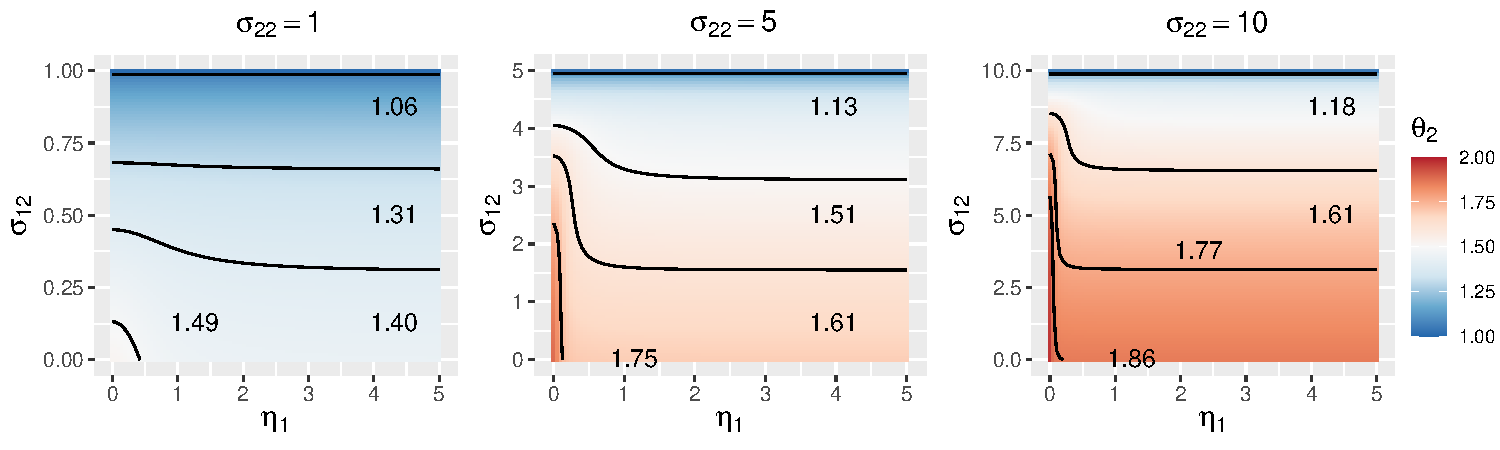
\includegraphics[width=0.95\linewidth]{bivariate_extcoef_rho_alpha.pdf}     
        \caption{}
        \label{fig:skewed_BR_extcoef}
    \end{subfigure}
    \begin{subfigure}{1\textwidth}
        \centering
        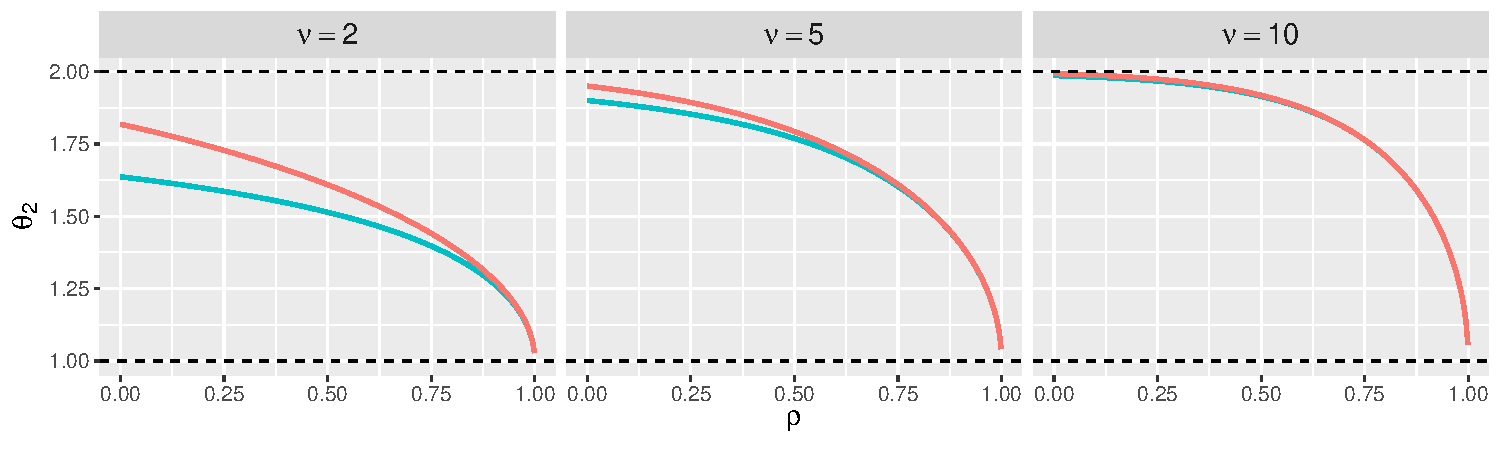
\includegraphics[width=0.95\linewidth]{bivariate_extcoef_truncT.pdf}    
        \caption{}
        \label{fig:truncated_extcoef}
    \end{subfigure}
    \caption{(a): Image plots of the bivariate extremal coefficient of the skewed Brown-Resnick model with parameters $\bm\eta = (\eta_1,-\eta_1)^\top$ and $\Sigma = ((\sigma_{22},\sigma_{12})^\top,(\sigma_{12},\sigma_{22})^\top)$ where $\sigma_{22} = 1,5$ and $10$ (left to right), as function of $\eta_1$ and $\sigma_{12}$. (b): Bivariate extremal coefficient of the truncated extremal-t process (blue) and the extremal-t process (red) with degrees of freedom $\nu=2,5$ and $10$ (left to right), as a function of the correlation parameter $\rho$.}
\end{figure}

From \eqref{eq:bi_extcoef_skewed_BR}, the bivariate extremal coefficient of the skew Brown-Resnick model depends on $\Sigma$ partly through $\gamma_{12}$, which corresponds to the semivariogram of the random vector $\bm Y$ defined in Theorem~\ref{thm:skewBR}. Whereas in the Brown-Resnick case, the extremal coefficient is fully characterised by the semivariogram.
%
Opting for a parametrisation based on semivariogram functions over covariance functions leads to greater interpretability of the model parameters and allows for asymptotic independence in the long range when considering an unbounded variogram. Indeed, taking the power-law semivariogram $\gamma(h) = (h/\lambda)^\vartheta$ for spatial lag $h$, where $\lambda>0$ and  $\vartheta \in (0,2]$ are respectively the range and smoothness parameters,
%while $h$ is the spatial lag, 
then as $h \rightarrow \infty$ we have $\bm \eta \equiv \bm \eta (h) \rightarrow \bm 0$ and therefore $\bm \xi = \bm \xi(h) \rightarrow \bm 0$ which implies that, in \eqref{eq:bi_extcoef_skewed_BR}, $\theta_2 \rightarrow 2$.
%

% However, as we see from \eqref{eq:bi_extcoef_skewed_BR}, the parameter $\Sigma$ is linked to the extremal coefficients via $\gamma_{12} = E[(W_1-W_2)^2]/2$, which is actually a semivariogram. 
% Therefore, using semivariogram functions is more interpretable than using covariance functions when fitting the (skewed) Brown-Resnick model as well as more flexible in the sense that it can bring asymptotic independence in the long range with unbounded variogram, e.g., the powered law semivariogram $\gamma(h) = (h/\lambda)^\nu$, where $\lambda$ is the range parameter, $\nu$ is the smoothness parameter, and $h$ is the distance. The construction of a stationary Brown-Resnick process using a nonstationary log-Gaussian process with an unbounded semivariogram was first introduced by \cite{Wadsworth.Tawn:2014}. 
Individually estimating the $D$ components of the parameter vector $\bm \eta$ under the constraint $\bm \eta^\top \bm 1=0$ is a difficult task. We therefore propose to represent $\bm \eta$ through spline functions. Consider the location $\bm s_i = (s_{i,1}, s_{i,2}) \in \mathcal{S}=\mathbb{R}^2$, $i=1, \ldots, D$. Let $\eta_i = \sum_{j=1}^J b_{j}K_j(\bm s_i)$, where $K_j(\bm s_i)$ is the $j$-th basis function evaluated at the location $\bm s_i$, and $b_j$ is the coefficient for the $j$th basis. The sum-to-zero constraint can be imposed by setting $\sum_{i=1}^D K_j(\bm s_i)=0$. As such, instead of trying to estimate every individual $\eta_i,i=1,\dots,D$ under the sum-to-zero condition, the coefficients $b_j,j=1,\dots,J$ for the basis functions are estimated, automatically satisfying the condition.
%
% As for the parameter $\eta$,  which is a vector with dimension $D$ and has a sum of zero. It is not very practical to estimate every component of $\eta$ individually and make it satisfy the sum-to-zero condition. Here, we use spline functions to represent the parameter $\eta$. We can write $\eta_i = \sum_{j=1}^J b_{j}B_j(\bm s_i)$, where $\bm s_i = (s_{1,i},s_{2,i})$ and $B_j(\bm s_i)$ is the $j$th basis function evaluated at the location $\bm s_i$, and $b_j$ is the coefficient for the $j$th basis. The sum-to-zero constraint can be imposed by setting $\sum_{i=1}^D B_j(\bm s_i)=0$. Therefore, instead of trying to estimate every individual $\eta_i,i=1,\dots,D$, and make sure that the sum-to-zero condition is satisfied, we can estimate the coefficients $b_j,j=1,\dots,J$ for the basis functions and the sum-to-zero condition will be automatically satisfied. 
In the remainder of this paper, $K_j(\cdot)$ denote Gaussian kernels centered at locations $\bm s_j^\star, j=1,\dots,J$, i.e.,
\begin{equation}
\label{eq:Gaussian_splines}
    K_j^\star(\bm s_i) = \phi\left(\frac{\|\bm s_i-\bm s_j^\star\|}{2\sigma_B}\right)-\frac{1}{D}\sum_{k=1}^{D}\phi\left(\frac{\|\bm s_k-\bm s_j^\star\|}{2\sigma_B}\right),\quad \text{and}\quad K_j(\bm s_i) = \frac{K_j^\star(\bm s_i)}{\sqrt{\sum_{k=1}^D K_j^\star(\bm s_k)^2}}.    
\end{equation}
%
Figure~\ref{fig:skewed_BR_extcoef_spatial} displays the bivariate extremal coefficient of the skewed Brown-Resnick model over a $[0,32]\times[0,32]$ grid, with respect to reference points labeled by a star with $J=2$, $\sigma_B = 64$ and $\eta_i = \sum_{j=1}^2 b_{j}K_j(\bm s_i) + 0.1\text{sgn}(s_{2,i}\geq 16)$, where $\bm s_1^\star=(8,8)$, $\bm s_2^\star=(24,24)$, and $\text{sgn}(\cdot)$ denotes the sign function. Note that the last term in $ \eta_i$ serves as background noise to ensure the parameter $\bm\xi = \frac{\Sigma\bm\eta}{\sqrt{1+\bm\eta^\top\Sigma\bm\eta}}$ is numerically identifiable. This is because 
%when 
multiplying $\bm\eta$ by a positive constant $c$, 
%$\bm\xi=\frac{\Sigma\bm\eta}{\sqrt{1/c^2+\bm\eta^\top\Sigma\bm\eta}}$ 
will not have numerically significant change on $\bm\xi$ as the $\bm\eta^\top\Sigma\bm\eta$ term will dominate the denominator, especially the nonstationarity introduced by the parameter $\bm\eta$ is not significant presented in the data.  
\begin{figure}[!t]
    \centering
    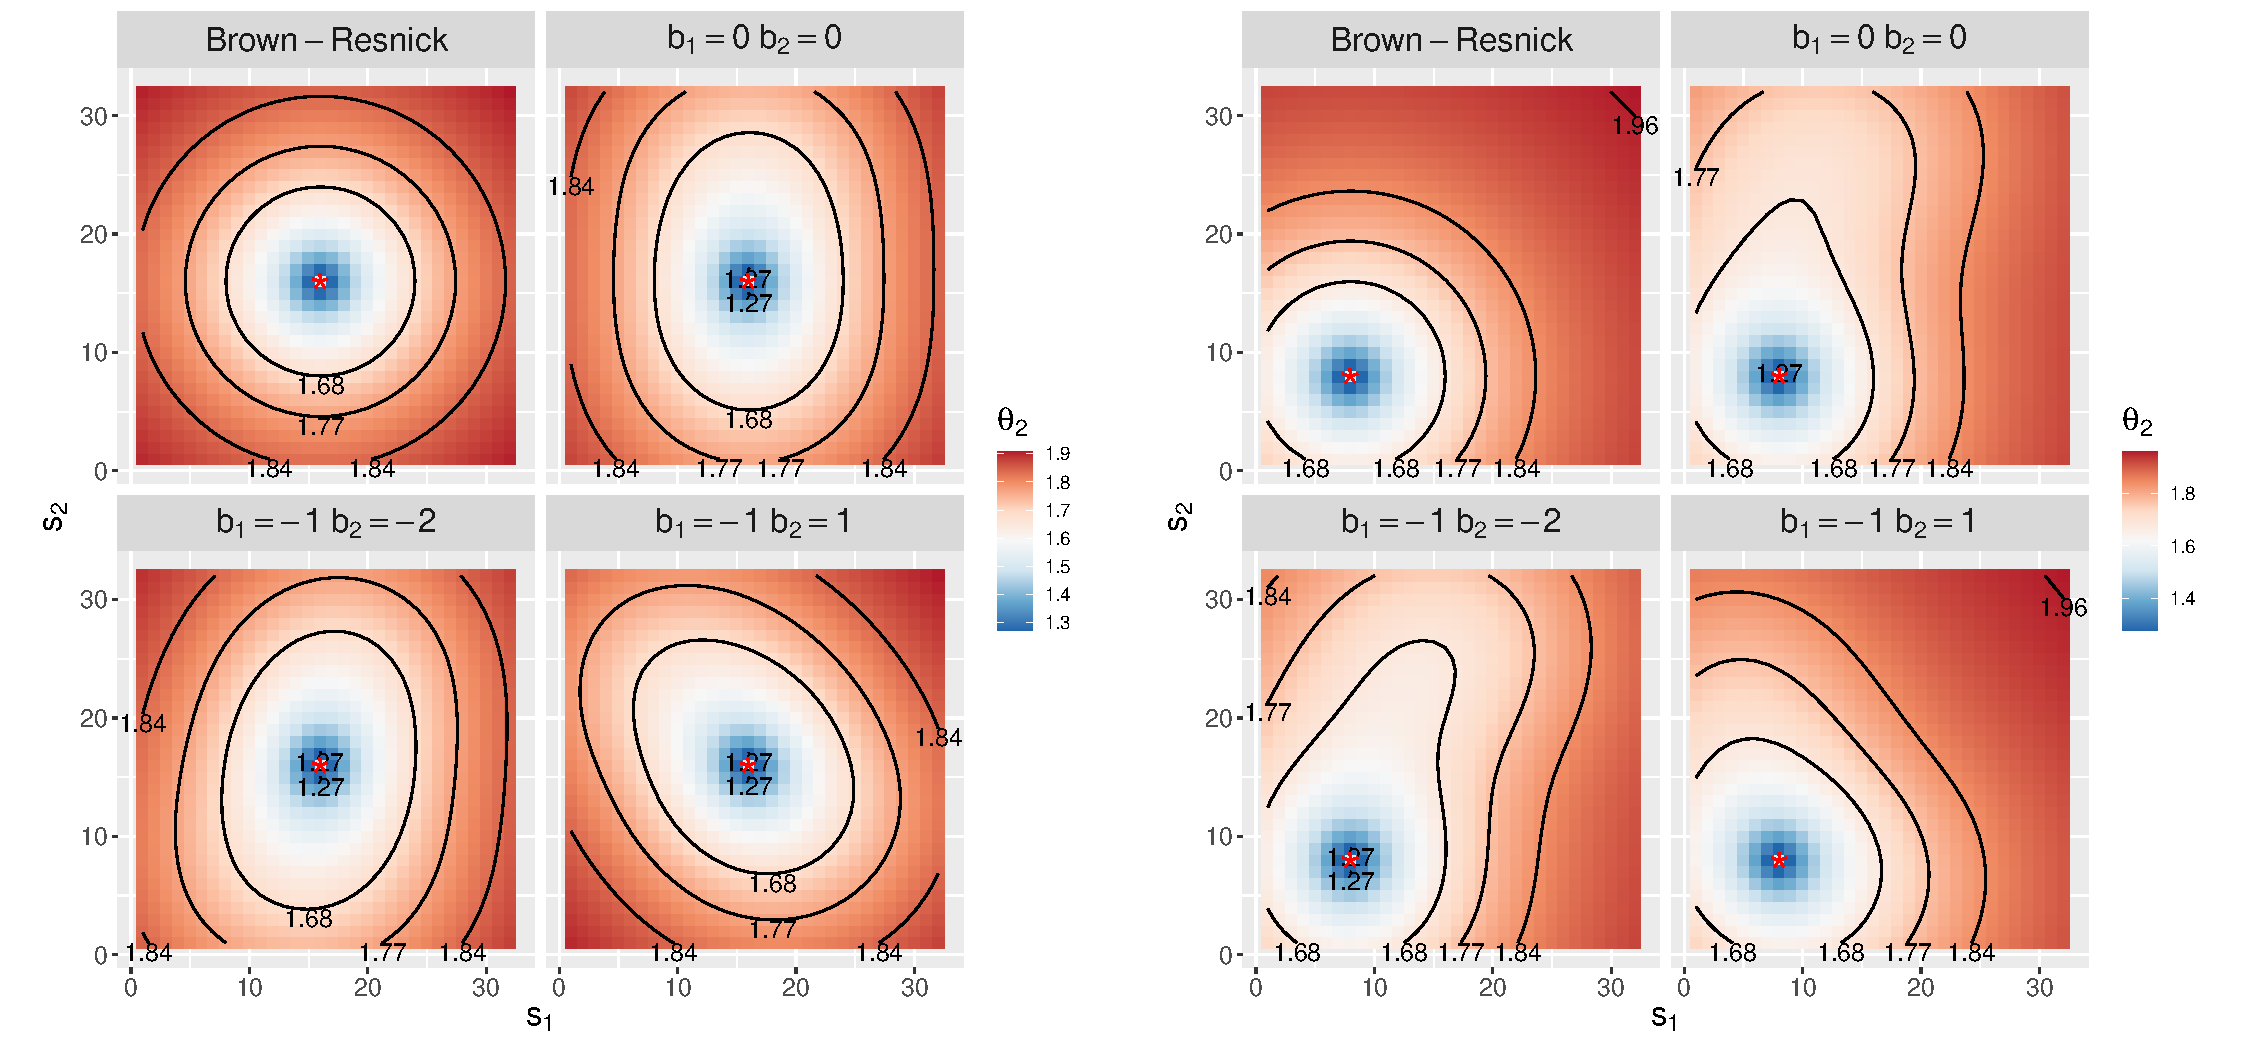
\includegraphics[width=1\textwidth]{extcoef_final_logskew.pdf}    
    \caption{Heatmaps and contour levels (solid black lines) of the bivariate extremal coefficient for the Brown-Resnick model ($\eta_i=0,i=1,\dots,D$) and skewed Brown-Resnick model where $\eta_i = \sum_{j=1}^2 b_{j}K_j(\bm s_i) + 0.1\text{sgn}(s_{2,i}\geq 16),i=1,\dots,D$ using $(b_1, b_2) = (0,0)$, $(-1,-2)$ and $(-1,-1)$. A star indicates a different basis function reference point between left and right panels.}
    \label{fig:skewed_BR_extcoef_spatial}
\end{figure}
Focusing on a single reference point (star), i.e.~on either the four left or right panels of Figure~\ref{fig:skewed_BR_extcoef_spatial}, we observe that varying the $\bm \eta$ vector through $(b_1, b_2)$ produces a broad range of dependence structures. Similarly, for fixed parameter values $(b_1,b_2)$, different dependence behaviours are observed depending on the reference point, putting the spotlight on an important feature of the skewed Brown-Resnick process: the ability to model non-stationarity. This important property, exhibited by numerous real-world environmental extreme phenomena, is due to the fact that \eqref{eq:bi_extcoef_skewed_BR} not only depends on the spatial lag between two locations, but also on the corresponding components of the $\bm \xi$ parameter vector. A similar observation was made by \citet{Beranger.etal:2017} about the extremal skew-t model.

%%%%%%%%%%%%%%%%%%%%%%%%%%%%%%%%%%
\section{Inference method} %%%%%%%
\label{sec:inference} %%%%%%%%%%%%
%%%%%%%%%%%%%%%%%%%%%%%%%%%%%%%%%%

From hereon we focus on the skewed Brown-Resnick model defined through \eqref{eq:V_skBR} with the power-law semi-variogram $\gamma(h) = (h/\lambda)^\vartheta$, $\lambda>0, \vartheta \in (0,2]$ and a spline representation of $\bm \eta$, and the truncated extremal-t defined through \eqref{eq:V_tet} with the power-exponential correlation function $\rho(h) = \exp(-(h/\lambda)^\vartheta)$, $\lambda>0$, $0 < \vartheta \leq 2$. 
Traditional likelihood-based inference methods for max-stable processes have only been feasible using composite likelihoods \citep{Padoan.etal:2010,Castruccio.etal:2016}, with $k$-th order log-likelihood function defined as
\begin{equation}
\label{eq:composite}
\ell_{C;k}(\bm \theta;\bm x_1,\dots,\bm x_n)=\sum_{S \in K_k; \forall K_k} \zeta_S \sum_{i=1}^n\log g(\bm x_{i,S};\bm \theta), \quad k< D,
\end{equation}
where the first summation is over all the subsets of $\{1,\ldots,D\}$ with cardinality $k$, $g(;\bm \theta)$ is the density associated with the $k$-dimensional distribution function $G(\cdot; \bm \theta)$ as defined in \eqref{eq:ppp}, $\bm x_{i,S}$ denotes the subvector obtained by restricting $\bm x_i$ to the components indexed by $S$, and $\zeta_S \geq 0$ are some weights. Due to the form of \eqref{eq:ppp}, the joint density function is expressed as,
\begin{equation*}
\label{eq:densitymaxstable}
    g(\bm x;\bm{\theta})=\exp\{-V(\bm x;\bm\theta)\}\sum_{\pi\in \mathcal P_D}\prod_{\tau\in \pi}\left\{-V_\tau(\bm x;\bm \theta)\right\},
\end{equation*} 
where $\mathcal P_D$ is the collection of all partitions $\pi=\{\tau_1,\ldots,\tau_{|\pi|}\}$ of the set $B_D$ (of cardinality $|\pi|$) and we recall that $V_\tau$ indicates the partial derivative of the function $V$ with respect to the variables indexed by the set $\tau$. The cardinality of $\mathcal P_D$ corresponds to the $D$-th Bell number, implying that the composite likelihood function is intractable even for moderate dimensions, making inference extremely challenging. Feasible attempts have mostly focused on pairs or triples \citep{Padoan.etal:2010, Huser.Davison:2013a} while \citet{Castruccio.etal:2016} considered higher orders up to $k=11$. \citet{Stephenson.Tawn:2005} offer an alternative solution relying on observations of the partition $\pi$, referred to as hitting scenarios \citep[see also][]{Wadsworth.Tawn:2014}. \citet{Beranger.etal:2021} combined both composite and Stephenson-Tawn likelihoods to propose fast and efficient inference for the extremal skew-t process. Most of the methods described above consider
% or $d=3$ \citep{Beranger.etal:2021} with 
$\zeta_S=1$ when the components in $S$ are within a disk of fixed radius and $\zeta_S=0$, otherwise. This cut-off distance 
% for the composite likelihood method to make the computation more feasible by 
removes terms in \eqref{eq:composite} whose components are far away from each other but the selection of this tuning parameter is not straightforward. 
% Even with the cut-off distance, the composite likelihood method is still computationally expensive for even moderate dimensions.  

As mentioned in Section~\ref{sec:intro}, the proposed methodology for inference of max-stable models is through \eqref{eq:angular_likelihood_1} which is based on the approach of  \cite{Coles.Tawn:1994} and only requires knowledge of the angular density function $h(\bm w)$. For models that only put mass on the interior of the simplex, this approach has immense potential for scalability to high dimensions since it only requires the evaluation of the angular density on $\Omega^\circ$ and avoids any other sub-spaces of $\Omega$. Theorem~\ref{thm:augular_density} establishes the conditions for a model to be fully defined by its density on $\Omega^\circ$ and Proposition \ref{prop:AngDesn_eT} \& \ref{prop:AngDesn_skBR} give a closed form expression for two new models. 
% As our models do not put mass on $\partial\Omega$, we only need to compute the angular density in the interior, $\Omega^\circ$. 
Given $n$ observations at $D$ spatial locations, $\bm x_1,\dots,\bm x_n$, and a threshold $r_0>0$, the approximate log-likelihood from \eqref{eq:angular_likelihood_1} becomes
%
\begin{equation}
\label{eq:angular_likelihood_2}
\ell_A(\bm \theta;\bm x_1,\dots,\bm x_n) = 
\sum_{i \in \{m: \|\bm x_m\| > r_0\}} 
\log\kappa\left(\frac{\bm x_i}{\|\bm x_i\|};\bm \theta\right). 
\end{equation} 
%
Unlike the composite likelihood estimates which are proven to be asymptotically unbiased and normally distributed, the estimates maximising \eqref{eq:angular_likelihood_2} are biased since the likelihood function is not the likelihood of the max-stable process itself but of a limiting Poisson process. The simulation experiments in the next section demonstrate that the bias can be controlled to an acceptable level by selecting an appropriate threshold $r_0$ and is dominated by the computational gains of the methodology.
% However, as I mentioned the composite likelihood is computationally expensive to fit, the ultimate gain by using the angular approximate likelihood is the computational efficiency. 
The angular density of the Brown-Resnick process is an extended skewed log Gaussian density function, which can be computed easily. For the truncated extremal-t processes, the angular density function is the truncated multivariate Student-t density after normalisation by $\bm a$. The main bottleneck is the evaluation of $\bm a$, which involves computation of the multivariate Student-t cdf, but the use of the R package \texttt{TruncatedNormal} \citep{Botev.Belzile:2021} can alleviate these issues (for dimensions up to 1000). Performance comparisons between the approximated and pairwise composite likelihood methods are conducted in the following sections.
%through extensive simulation studies.
% In the next session, we will do extensive simulation studies to compare the performance of the approximate likelihood method with the composite likelihood method.       

%%%%%%%%%%%%%%%%%%%%%%%%%%%%%%%%%%%%
\section{Simulation Study} %%%%%%%%%
\label{sec:sim} %%%%%%%%%%%%%%%%%%%%
%%%%%%%%%%%%%%%%%%%%%%%%%%%%%%%%%%%%

We first establish exact simulation algorithms to generate from skewed Brown-Resnick and truncated extremal-t processes, based on extremal functions \citep{Dombry.Engelke.Oesting:2016}. These are detailed in Sections~A.4 and B.4 of the Supplemental Material. On a $15\times15$ grid (i.e., $D=225$),  we generate 500 observations from the Brown-Resnick model with $\lambda=3,6$ and $\vartheta=0.5,1,1.5$ (6 combinations), and 2000 observations from the skewed Brown-Resnick model with $\lambda=5,10$, $\vartheta = 1,1.5$, and $(b_1,b_2) = (0,0),(-1,-2),(-1,1)$ (12 combinations), where the centres of the kernels are chosen to be $\bm s_1^\star = (4,4)$ and $\bm s_2^\star=(11,11)$. Finally, we generate 2000 observations from the truncated extremal-t on a $10\times10$ grid (i.e., $D=100$) with $\lambda=1,3$, $\vartheta=1$ and $\nu=2$ (3 combinations). Parameters are estimated by maximising the composite and approximate likelihoods, respectively \eqref{eq:composite} and \eqref{eq:angular_likelihood_2}, and the procedure is repeated 300 times.
% and we repeat this process for 300 times. Therefore, in total, there will be 6 cases of different combinations of $\nu$ and $\lambda$. 

For the approximate likelihood, the higher the threshold $r_0$ the better the Poisson approximation to the true likelihood, but simultaneously the fewer observations available. Taking this trade-off into consideration, choosing a threshold of
%the threshold is chosen to be 
$r_0 = 30\times D$ for the Brown-Resnick model
% as the data are marginally unit Fr\'echet distributed and $30$ is approximately the $96.7\%$ quantile in the unit Fr\'echet scale, which 
results in retaining about $16$ observations while choosing $r_0 = 100\times D$ for the skewed Brown-Resnick model results in about 20 observations retained. The impact of the threshold is investigated for the truncated extremal-t where the threshold is set to the $90\%, 95\%$, and $98\%$ quantiles of the observed radial components. For the composite likelihood, we use the pairwise likelihood, $\ell_{C;2}$ in \eqref{eq:composite}, where $\zeta_S$ takes the value $1$ if the distance between pairs is less than or equal to $2\sqrt{2}\approx 2.83$ and $0$ otherwise, yielding $2268$ pairs for likelihood calculation.
%to be included in the likelihood. 



We first establish the baseline performance of the approximate likelihood versus pairwise composite likelihoods for a standard model.
Figure~\ref{fig:simulation_boxplot_BR} displays violin plots of the 300 replicate estimated parameters $\hat\lambda$ and $\hat\vartheta$ from the Brown-Resnick model using  approximate (red) and composite likelihoods (blue), where true parameter values are indicated by dots. 
Overall, performance is as expected.
%Globally the proposed methodology appears to be performing well, admittedly the pairwise composite approach seems more stable. As expected, 
The estimates obtained from maximising \eqref{eq:angular_likelihood_2} exhibit some bias, in particular for the range parameter ($\lambda$), especially for case 5 ($\lambda=3, \vartheta=1.5$) where the Brown-Resnick process possesses a weaker dependence structure. There is also greater variability in the approximate likelihood estimates compared to the composite likelihood estimates, which are generally unbiased and relatively precise. The bias in the approximate likelihood will reduce as the threshold $r_0$ increases (see e.g.~Figure \ref{fig:simulation_boxplot_truncT}, below), although in practice increasing thresholds will reduce the data available for model fitting.
%
%In this case, the angular approximate likelihood might need more data (if possible) and/or a higher threshold to diminish the bias. 
%
%The range of the relative bias $\hat\lambda/\lambda$ is $[7.3\%-20.7\%]$ when using the approximate likelihood and down to $[0.001\%-0.257\%]$ when opting for the composite likelihood. Similarly, the range of the relative bias $\hat\vartheta/\vartheta$ ranges reduces from $[1.5\%-9.7\%]$ to $[0.015\%-0.087\%]$. 
% for $\hat\nu$, whereas the pairwise likelihood only have relative biases ranging from $0.014\%$ to $0.25\%$. 
%Even though, for the selected sample size and threshold, the angular approximate likelihood does not provide estimates as accurate as the pairwise likelihood, its computational efficiency is far superior. 
However, the approximate likelihood estimator is by far the most computationally efficient.
A model fit based on the composite likelihood takes an average of 13.6 minutes across all cases (on a 16-core machine), whereas it only takes 20.9 seconds using the angular density, which is about 39 times faster. As dimension ($D$) increases, we can expect the relative performance of the approximate to the composite likelihood to improve due to more available data (higher $r_0$, so less bias) and more terms in the composite likelihood.
\begin{figure}[ht]
    \centering
    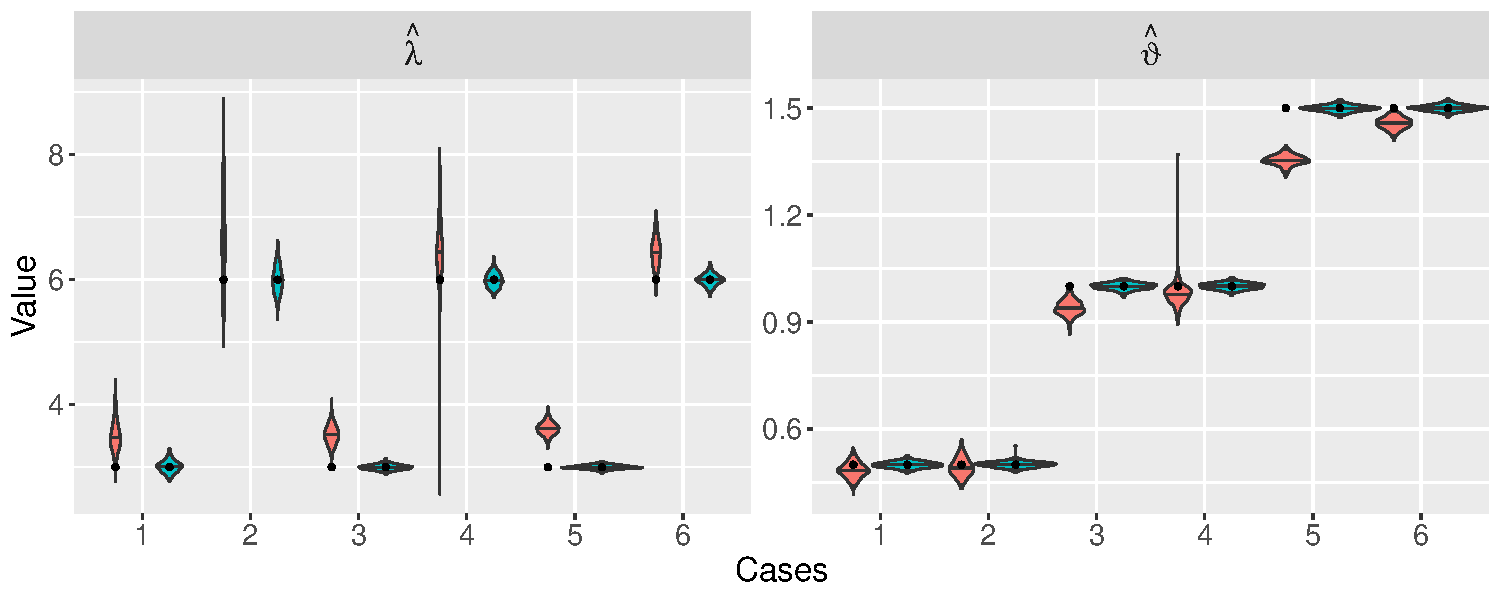
\includegraphics[width=1\textwidth]{simulation_est_boxplots_final_BR_30.pdf}    
    \caption{Violin plots for 300 replicate estimates of $\bm \theta = \left(\lambda, \vartheta\right)$ for the Brown-Resnick process with $\lambda=3,6$ and $\vartheta=0.5,1,1.5$ using the approximate likelihood (red) and the pairwise likelihood (blue) with 2268 pairs. Black dots indicate the true values.}
    \label{fig:simulation_boxplot_BR}
\end{figure}

We now examine estimation performance for the new models. 
Figure~\ref{fig:simulation_boxplot_truncT} shows violin plots for the estimates of the range and smoothness parameters 
%(respectively $\lambda$ and $\vartheta$) from 
for the truncated extremal-t model, where the degree of freedom is fixed at its true value ($\nu=2$), and the threshold $r_0$ is chosen to be the $98\%$ (red), $95\%$ (green), and $90\%$ (blue) empirical quantiles of the radial component. 
For the sample size of $n=2000$ observations, retaining the $2\%$ of observations (i.e., 40) with the largest radial components produces almost unbiased estimates. Lowering this threshold increases the bias but also increases the computation time since more observations are included. As highlighted in Section~\ref{sec:theory}, fitting the truncated extremal-t model requires more computational effort than the skew Brown-Resnick model,  here 
%it is observed that each model fit takes 
requiring a mean of about 15 minutes on a $10 \times 10$ grid ($D=100$).
%
Note that it is impractical to use composite likelihoods for the truncated extremal-t model as the marginal 
distribution of a multivariate truncated normal is not a truncated normal. This necessitates a costly numerical integration for each composite likelihood term \citep{Horrace:2005}. 
\begin{figure}[t]
    \centering
    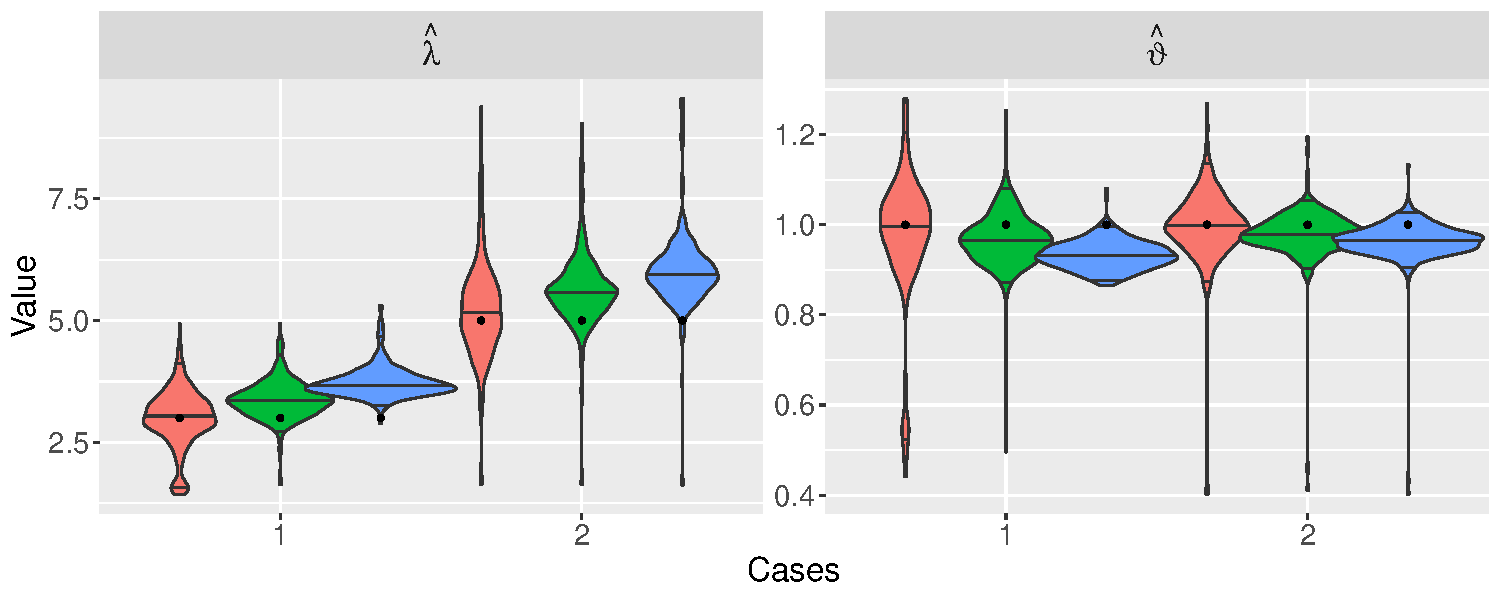
\includegraphics[width=1\textwidth]{simulation_est_boxplots_final_truncT.pdf}    
    \caption{Violin plots for 300 estimates of $\bm \theta = (\lambda, \vartheta, 2)$ for the truncated extremal-t process with $\lambda=3,6$, $\vartheta=1$, and $\nu=2$, using the approximate likelihood. The threshold $r_0$ is set to be the $98\%$ (red), $95\%$ (green) and $90\%$ (blue) empirical quantiles of the radial component. Black dots indicate the true values.}
    \label{fig:simulation_boxplot_truncT}
\end{figure}


Figure~\ref{fig:simulation_boxplot_skewedBR} shows parameter estimates for the skew Brown-Resnick process using the approximate likelihood, for the 12 parameter combinations. The estimates for $\lambda$ and $\vartheta$ are more accurate than those estimates shown in Figure~\ref{fig:simulation_boxplot_BR}, due to the larger sample size and higher threshold $r_0$. In particular, the estimates of the skewness-related parameters $(b_1,b_2)$ are all identifiable and almost unbiased.
Model fitting is computationally efficient, with each fit taking around $6$ minutes. 
%The optimisation process is implemented in three stages; first, the model is fitted holding $b_1=b_2=0$ fixed. Then, fixing $\lambda$ and $\vartheta$ at their estimated values, estimates are obtained for $b_1$ and $b_2$. Finally, the model is fitted one last time with $b_1$ and $b_2$ fixed at their estimated values. This approach helps avoid becoming trapped in local optima and improve the stability of the estimation procedure.    

\begin{figure}[t]
    \centering
    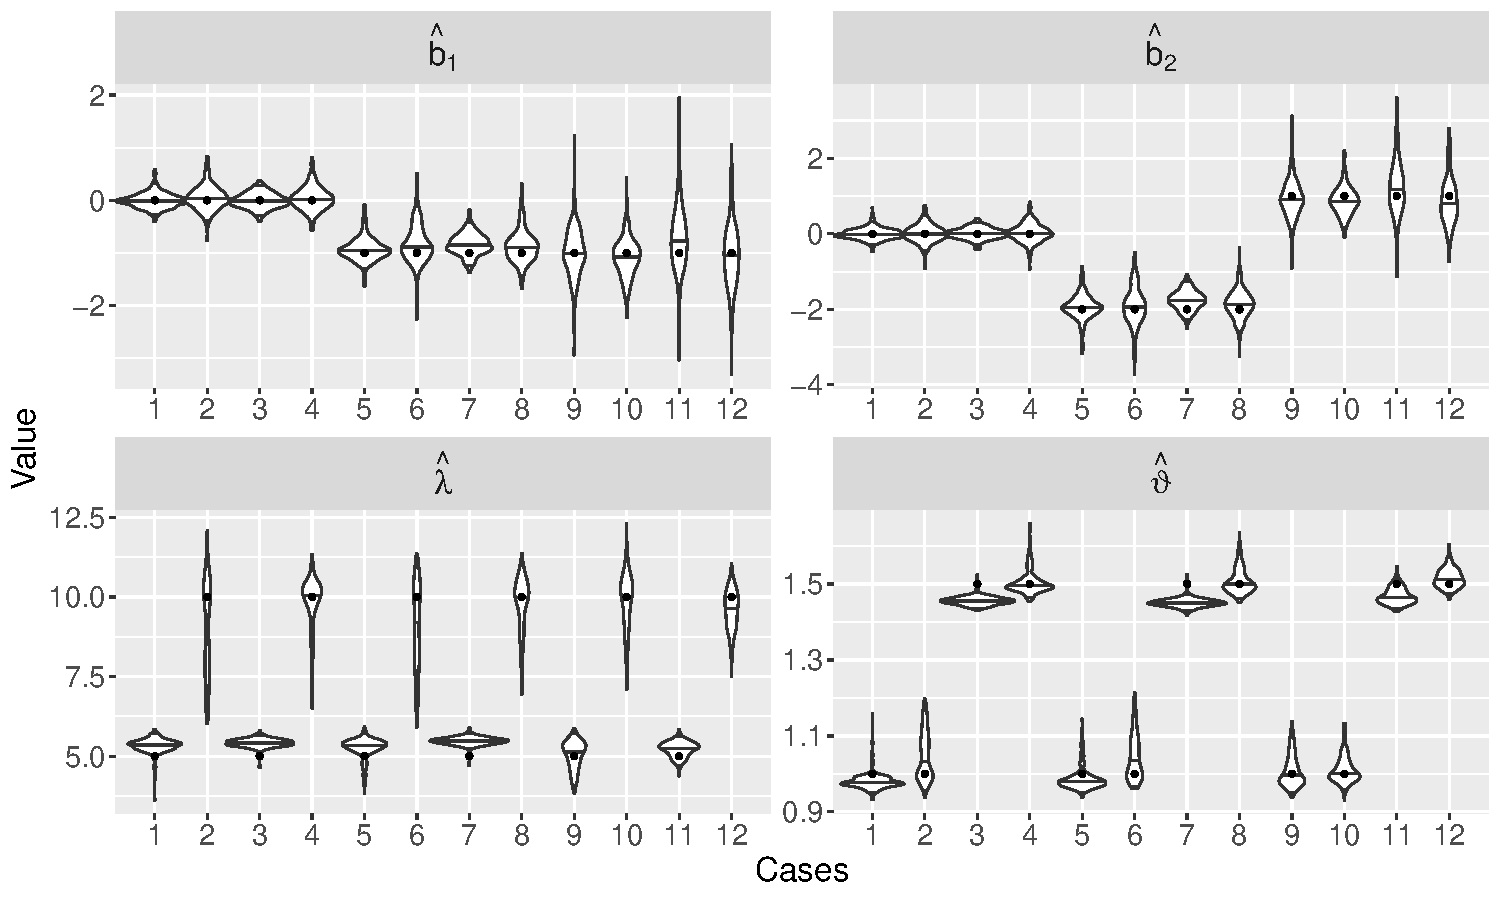
\includegraphics[width=1\textwidth]{simulation_est_boxplots_final.pdf}    
    \caption{Violin plots for the 300 estimates of $\bm \theta= \left(\lambda, \vartheta,  b_1, b_2\right)$ for the skewed Brown-Resnick process with $\lambda=5,10$, $\vartheta=1,1.5$, and $(b_1,b_2) = (0,0),(-1,-2),(-1,1)$, using the approximate likelihood. Black dots indicate the true values.}
    \label{fig:simulation_boxplot_skewedBR}
\end{figure}
\begin{figure}[t]
    \centering
    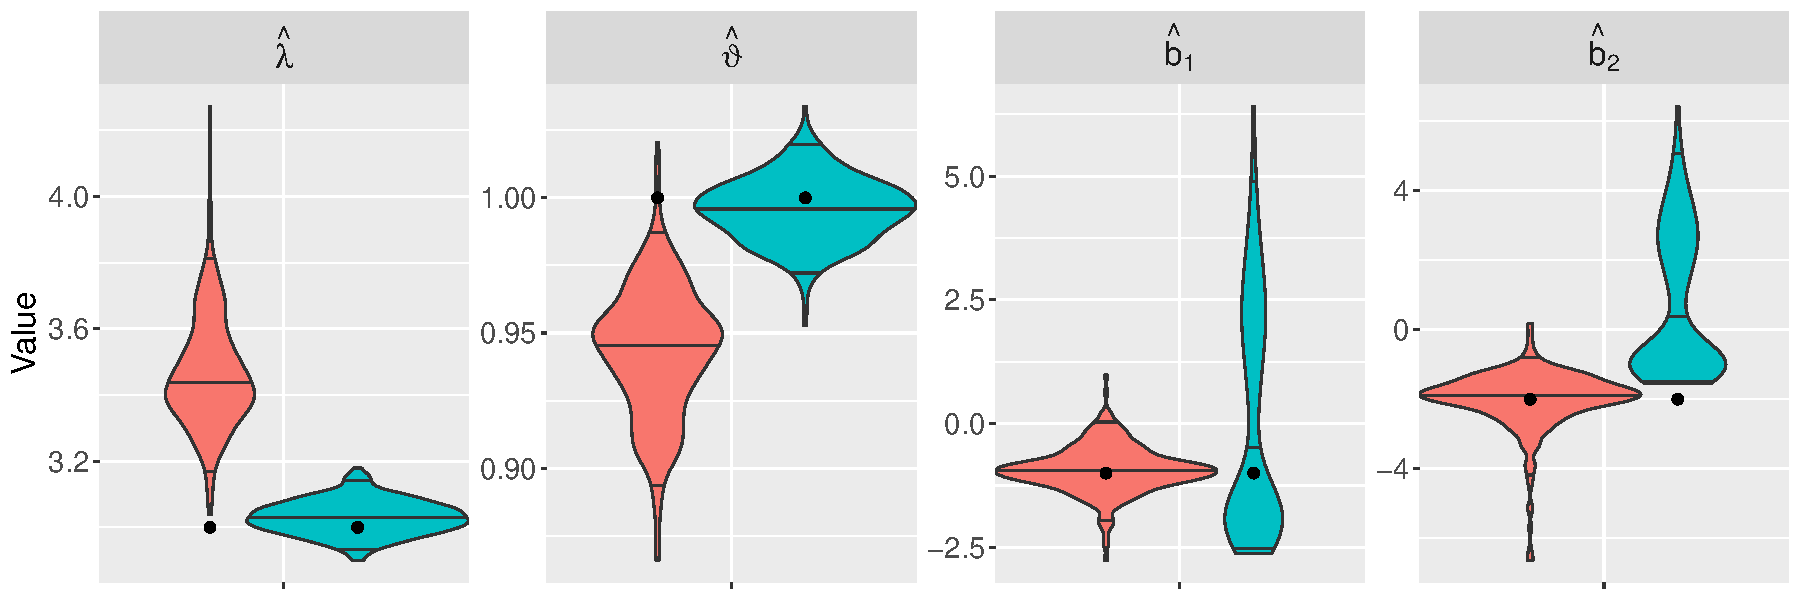
\includegraphics[width=1\textwidth]{simulation_est_boxplots_final_skewBR_comp.pdf}
    \caption{Violin plots for 300 estimates of $\bm \theta = (\lambda, \vartheta, b_1, b_2)$ for the skewed Brown-Resnick process with $\lambda=3$, $\vartheta=1$, and $(b_1,b_2) = (-1,-2)$ using the approximate likelihood (red) with threshold $r_0=30\times D$ and the pairwise likelihood (blue) with 1202 pairs. Black dots indicate the true values.}
    \label{fig:simulation_boxplot_skewedBR_comp}
\end{figure}


In contrast to the approximate likelihood, we found the composite likelihood estimators of  $b_1$ and $b_2$ for the skewed Brown-Resnick model to be 
%found to be 
unreliable.
%for the estimates of $b_1$ and $b_2$. 
As an illustration, we performed a small comparative study 
%study to compare the performance of the approximated likelihood approach with the pairwise likelihood approach for the skewed Brown-Resnick model 
based on datasets of 500 observations with parameters $\lambda=3$, $\vartheta=1$, and $(b_1,b_2) = (-1,-2)$, generated on the same $15\times15$ grid, and with the same kernel centres. 
%The kernels centers are chosen to be the same as the previous simulation study. 
As we have fewer observations (for computational tractability) we choose a 
%lower 
threshold of $r_0 = 30\times D$ for the approximate likelihood approach. For the pairwise likelihood, we use the 1202 closest pairs for likelihood calculation due to the computational overheads. 
%Then, unlike previous three-stage optimisation method, we estimate all the four parameters together by maximising the approximated likelihood and the pairwise likelihood with initial values set to be the true values to avoid local optima during optimisation, and we repeat the procedure for 300 times. 
Figure~\ref{fig:simulation_boxplot_skewedBR_comp} shows the 300 replicate estimates of $\lambda$, $\vartheta$, $b_1$, and $b_2$ for both approximate and pairwise likelihoods. The approximate likelihood provides almost unbiased estimates for the parameters $b_1$ and $b_2$ and the expected small relative bias (around $10\%$) for $\lambda$ and $\vartheta$.
%, which while be 
%can reduced with a higher threshold as seen above.
In contrast, the pairwise likelihood provides unbiased estimates for $\lambda$ and $\nu$, but biased estimates with large variability for $b_1$ and $b_2$.
%making the estimates indistinguishable from zero. 
The pairwise likelihood is also more computationally expensive, taking around 2.36 hours on average using a 16-core machine, compared to 124.4 seconds on average for the approximate likelihood using a single core. 


The experiments conducted in this section indicate that, for an appropriately selected threshold, the approximate likelihood approach can produce almost unbiased estimates with accuracy comparable to, and better than (for the skewed Brown-Resnick) the pairwise likelihood, at the fraction of the computational cost.    



\section{Application}
\label{sec:application}

We now examine the spatial dependence structure of
the sea surface temperature (in $^\circ \textrm{C}$) over the Red Sea, as previously considered by \cite{Huser.Zhong:2023}.
The data comprise 31 annual maxima observations recorded at $D=1043$ gridded locations from 1985 to 2015. 
We follow \cite{Huser.Zhong:2023} and standardise the margins to the unit Fr\'echet scale.
%The extremal dependence structure within these data have been analysed by \cite{Huser.Zhong:2023} and we therefore adopt the same marginal model for marginal standardisation to unit Fr\'echet scale.
%
The Brown-Resnick and its skewed alternative are fitted using the approximate likelihood with a threshold $r_0=10\times D$, where 10 approximately corresponds to the $90\%$ quantile of a unit Fr\'echet distribution, leaving 9 observations for model fitting.
%approximately and the threshold $r_0$ leaves 9 observations for likelihood calculation. 
A similar spline representation of $\bm\eta$ to the simulation study is chosen, where $J=5$, and the kernel centres $\bm s_j^\star, j=1, \ldots, J$ are selected in the middle of the Red Sea, along the north-south axis, shown as the black dots in Figure~\ref{fig:extcoef_application}. We implement no background noise, so that $\eta_i=0, i=1, \ldots, D$, as only $\bm\xi$ needs to be estimated (instead of $\bm\eta$) and so the identifiability of $b_i,i=1,\dots,J$ is not a concern. Parameter estimates below indicate that the parameters are identifiable,
%Jackknife parameter estimate standard deviations below indicate that we are able to %idenfity all the parameters reasonalely well, which is 
%likely 
due to the large number of locations and kernel spline used.

For the Brown-Resnick model, the parameter estimation takes $195$ seconds on a single core, yielding $\left( \hat{\lambda}, \hat{\vartheta}\right) = \left(68.97, 1.19\right)$ with jackknife standard deviations $(2.38,0.05)$. In comparison, the method of \cite{Huser.Zhong:2023}, relying on the pairwise composite likelihood with less than 2000 pairs, takes $31$ seconds using 32 cores while fixing the smoothness parameter $\vartheta$. In that context, with fixed $\vartheta$ the approximate likelihood takes $57$ seconds using a single core and produces similar results. The skewed Brown-Resnick estimates are $\left( \hat{\lambda}, \hat{\vartheta}, \hat{b_1}, \hat{b_2},\hat{b_3},\hat{b_4},\hat{b_5}\right) = \left(53.57, 1.37, -0.42, 0.58, -0.24, -0.18, 0.29\right)$, which were obtained in 39.5 minutes using 12 cores.
%with the three-stage optimisation method. 
The estimated $\hat\lambda$ is smaller but the estimated $\hat\vartheta$ is larger than the corresponding estimates for the Brown-Resnick model, which is to be expected as the estimated skewed Brown-Resnick model more properly accounts for the dependence strength and structure compared with the Brown-Resnick model. The corresponding estimated standard deviations based on the jackknife are $(1.68, 0.06, 0.13, 0.18, 0.07, 0.18, 0.27)$, suggesting that several of the the estimated slant parameters 
%$\hat{\bm\eta}$ 
are significantly different from zero. Finally, since the two models are nested, the Akaike Information Criterion can be used for model selection, confirming a better fit when including skewness in the distribution of the underlying process (AIC=-16458.04 versus -16430.1 for the Brown-Resnick).  

Maps of the bivariate extremal coefficient from the fitted Brown-Resnick and skewed Brown-Resnick models are given in the left and middle panels of Figure~\ref{fig:extcoef_application} for two reference locations (top and bottom rows). The right panels display empirical estimates which indicate the presence of some non-stationarity. The shape of the dependence structure estimated by the skewed Brown-Resnick model appears more realistic and better reflects the empirical observations. For example, there seems to be a region in the north of the Red Sea that is mildly dependent on the second reference point (bottom right panel) which is well captured by the skewed Brown-Resnick model (bottom left), and not at all by the Brown-Resnick model. 
\begin{figure}[ht]
    \centering
    \includegraphics[width=0.95\textwidth,page=11]{extcoef_application_2.pdf}
    \includegraphics[width=0.95\textwidth,page=18]{extcoef_application_2.pdf}
    \caption{Maps of bivariate extremal coefficient with respect to the centre labeled by the asterisk symbol for fitted skewed Brown-Resnick 
    %model 
    (left) and 
    %fitted 
    Brown-Resnick (centre) models 
    %(center) 
    with contours showing the same values in both panels. Right panels show the empirical bivariate extremal coefficient map. Black dots are the kernel centres used in the skewed Brown-Resnick model.}
    \label{fig:extcoef_application}
\end{figure}

\section{Discussion}
We have proposed a new estimation procedure for max-stable processes which relies on the angular density and avoids computing partial derivatives of the exponent function, the number of which quickly becomes intractable as the dimension of the data increases. In particular, the methodology can easily be applied to very high dimensional data under the condition that the angular density only puts mass on the interior of the unit simplex $\Omega$ and, as such, we have established general conditions for a model to possess such property. The well-known Brown-Resnick process falls within this family of models and we derive two new models: the \emph{skewed Brown-Resnick}, an extension of the Brown-Resnick that can model non-stationarity, and the \emph{truncated extremal-t}, the equivalent of the extremal-t but without mass on the subspaces of the simplex.  

Our simulation experiments have verified that, given an appropriately chosen threshold for the radial component, the approximate likelihood can perform as well as the pairwise composite likelihood and in some instances better. The statistical efficiency of the methodology is paired with its computational efficiency which allows it to fit flexible max-stable models to dimensions above 1000, as illustrated on a real dataset, within a reasonable timeframe. The advantages of the proposed methodology over the recent work of \citet{Huser.Zhong:2023} are also highlighted. Overall, this approach will help expand the usability of max-stable models in practice (when justified).  

The new models introduced in this manuscript are a step towards building spatial extreme models suited for real-world problems. Max-stable processes are closely related to r-Pareto processes \citep{deFondeville.Davison:2018} whose density is proportional to the intensity function of its corresponding max-stable process. r-Pareto processes models extreme data over a high threshold defined by a risk functional which, unlike max-stable processes, represents actual observations of a process and leaves more data for inference. Future work includes extending our models to r-Pareto processes and developing a framework for the delicate exercise of threshold selection.

\section*{Supplemental Material}
The Supplemental Material contains the proofs of the theorems and propositions, and the exact simulation algorithms for the skewed Brown-Resnick and truncated extremal-t models. The code for the simulation study and the application is available at \url{https://github.com/PangChung/InteriorExtremes}. 

\bibliographystyle{biometrika}
\bibliography{Total.bib}
\end{document}
